\section{L-FOCI in Generic ML Settings}
\begin{figure}
    \centering
    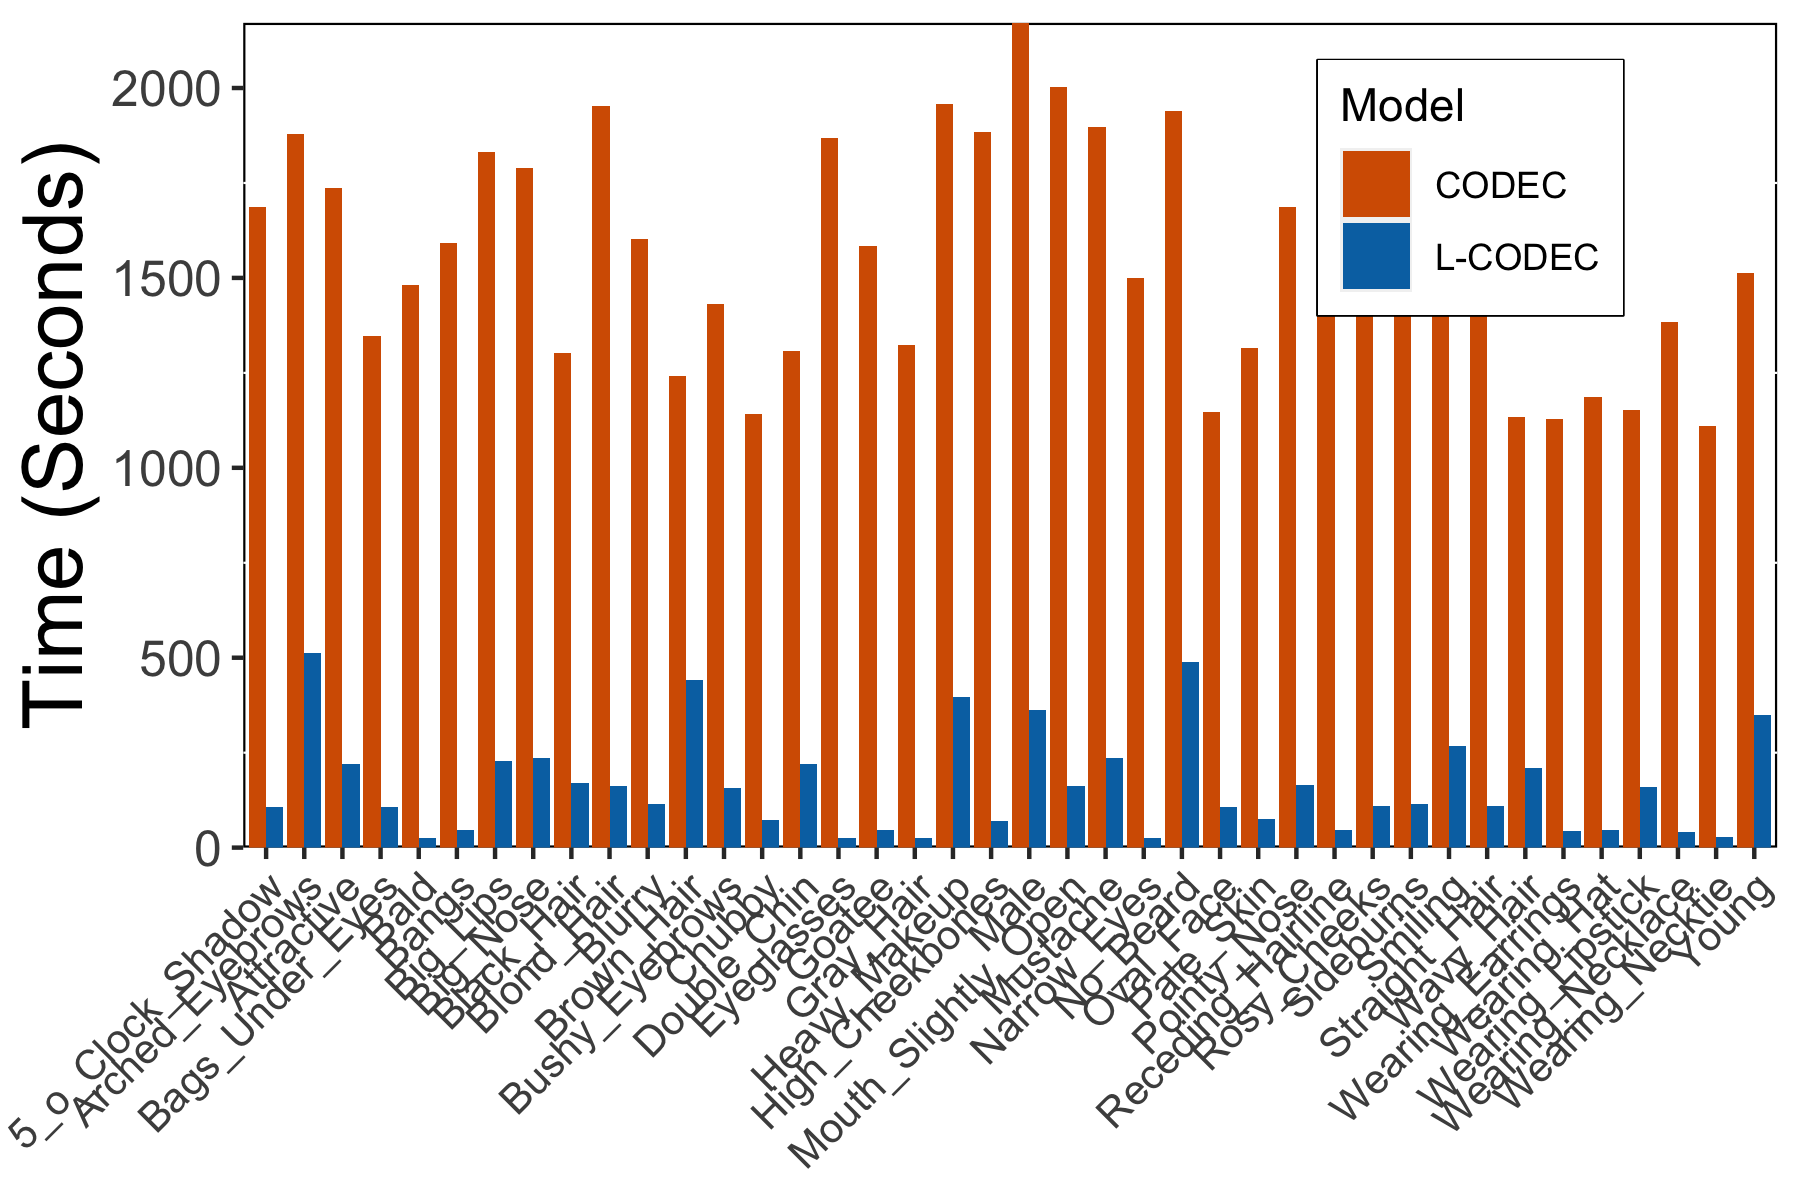
\includegraphics[width=0.98\columnwidth,trim={0, 11.6cm, 0, 0},clip]{5_unlearn/figs/Speed_Hist.png}
    \vspace{-8pt}
    \caption{\label{fig:speed_hist} L-CODEC vs CODEC run time comparison for identifying sufficient subsets for each CelebA attribute separately (pairs of columns, details in supplement).}
\end{figure}
We begin with understanding the value of L-CODEC and L-FOCI for Markov Blanket Identification and progress to applications
% Once their use has been properly justified in simpler, more direct applications, we demonstrate the value directly 
in typical unlearning tasks involving large neural networks previously infeasible with existing scrubbing tools.
See appendix for additional details. 
%Our code is at \url{https://github.com/xxx-xxxx/}.

% \subsection{L-FOCI in Generic ML Settings}
% \begin{figure}
%     \centering
%     %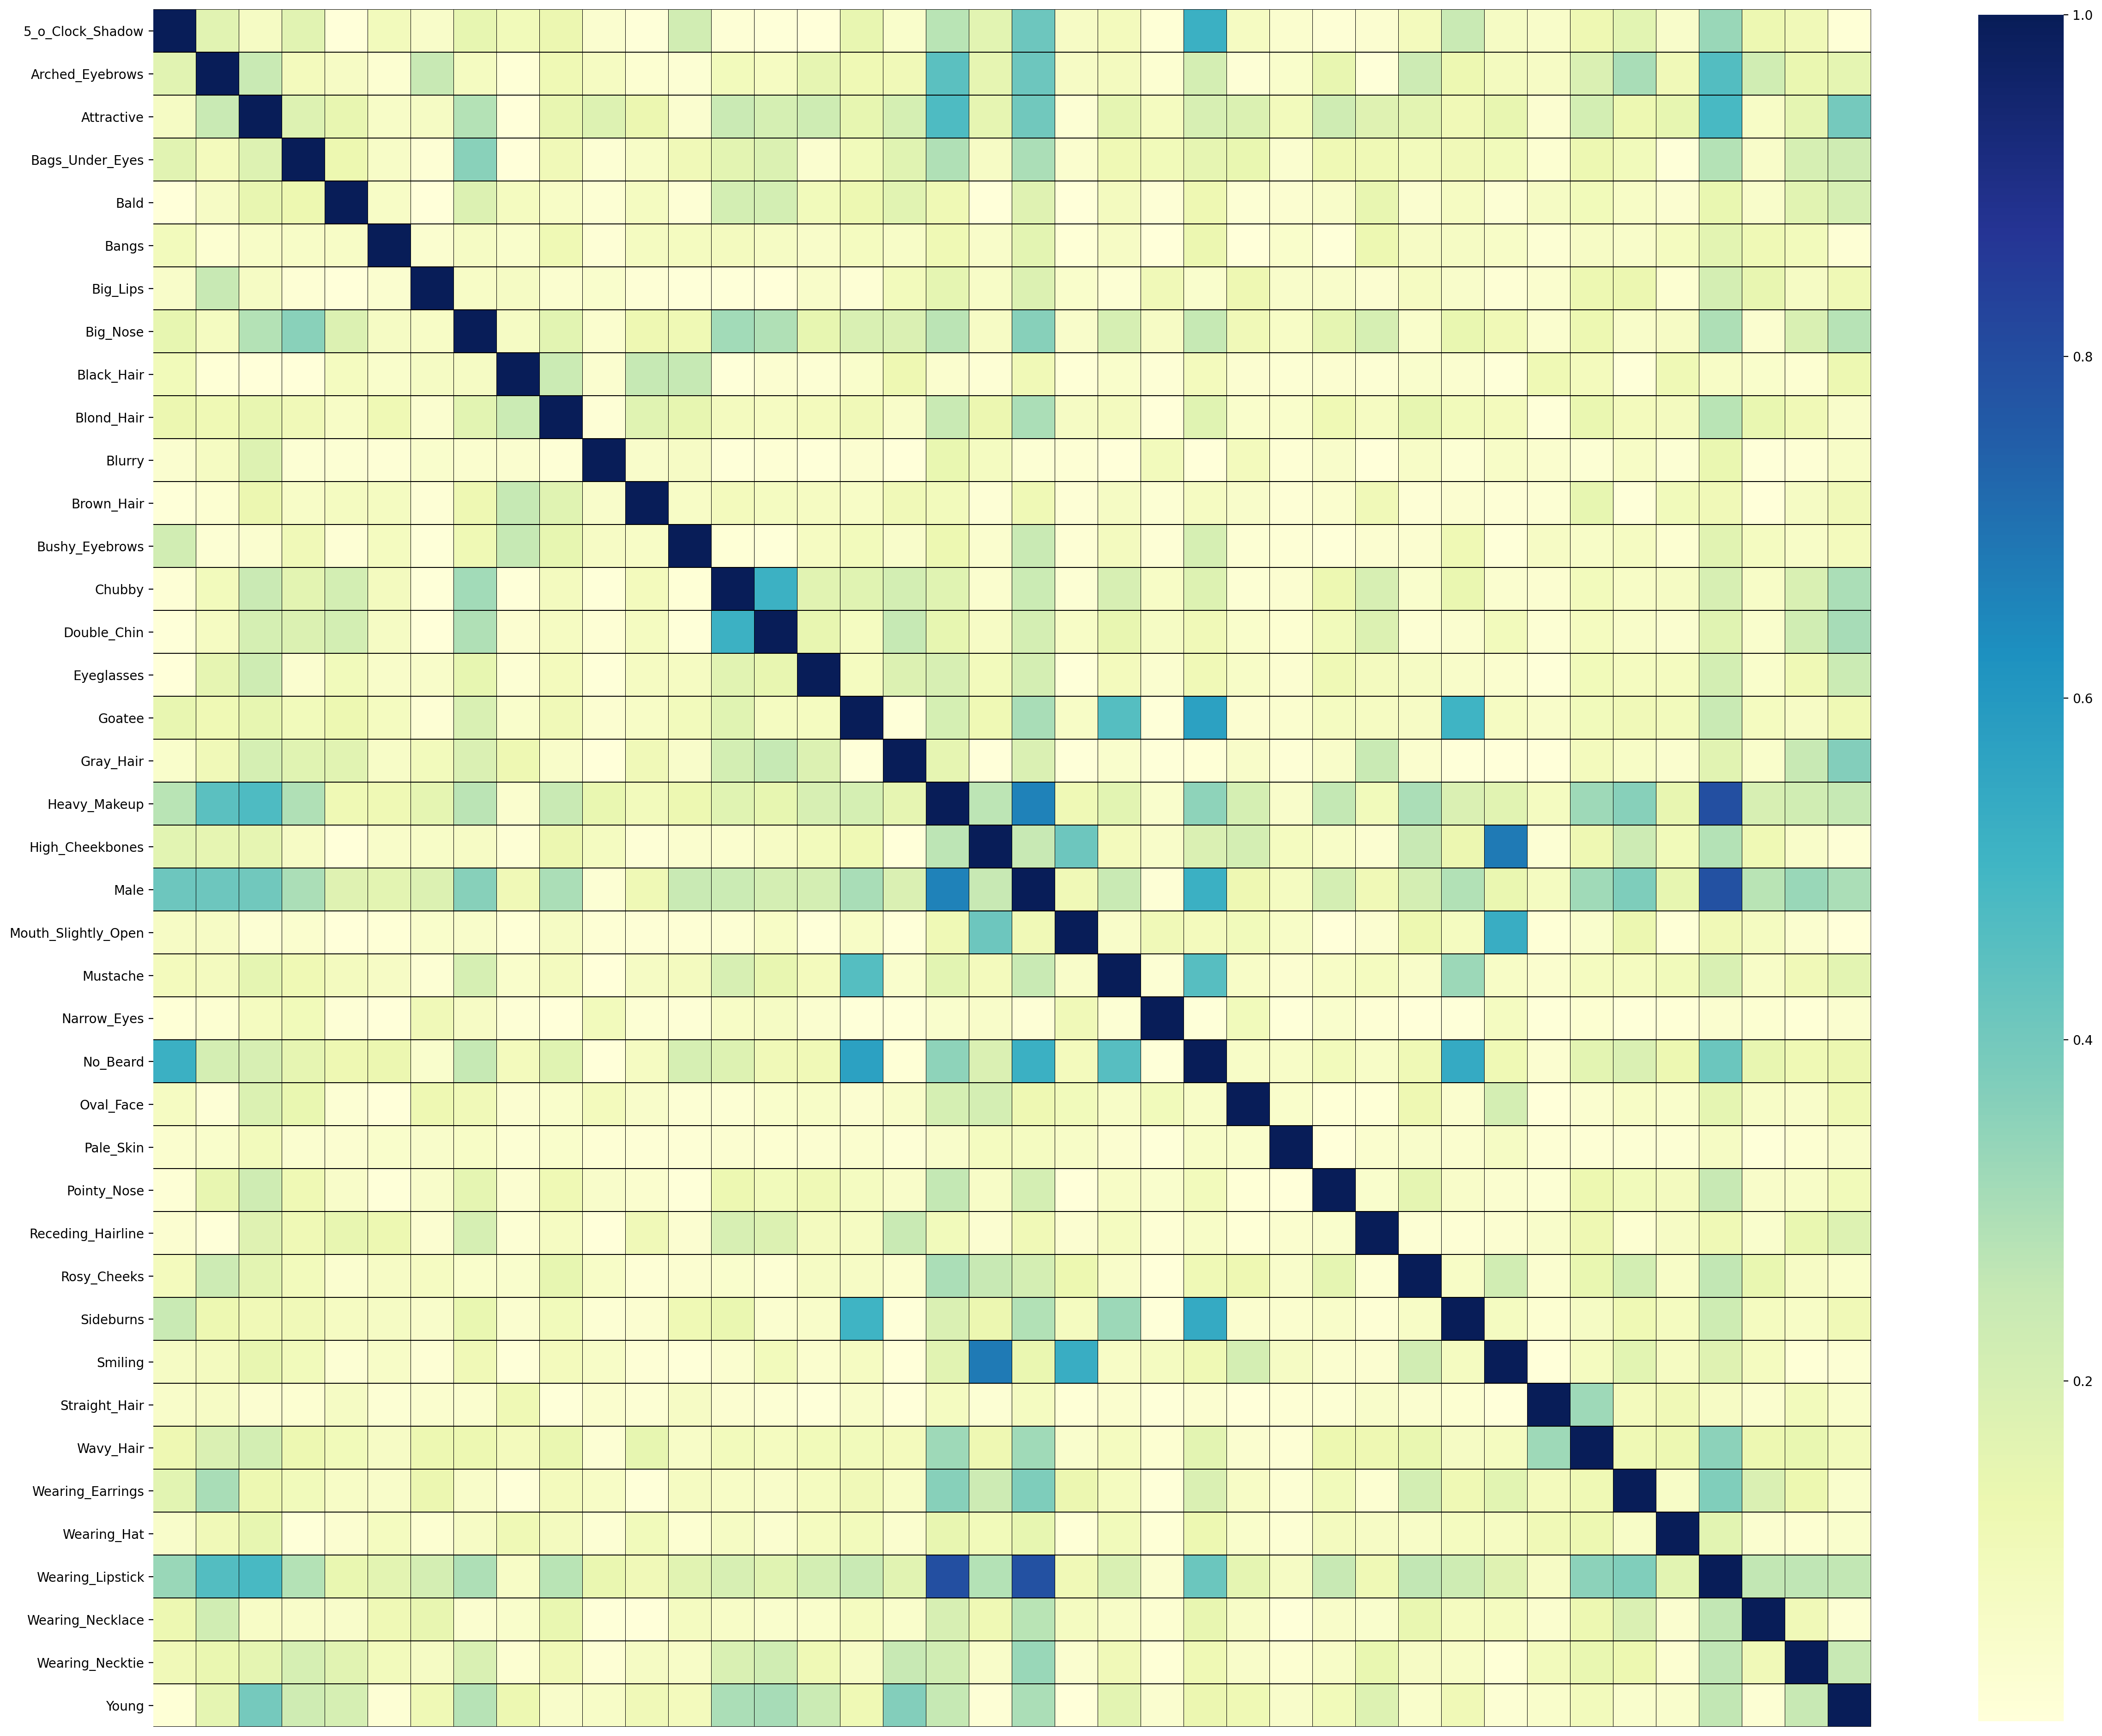
\includegraphics[width=0.25\textwidth]{figs/Pearson_noise_0.png}
%     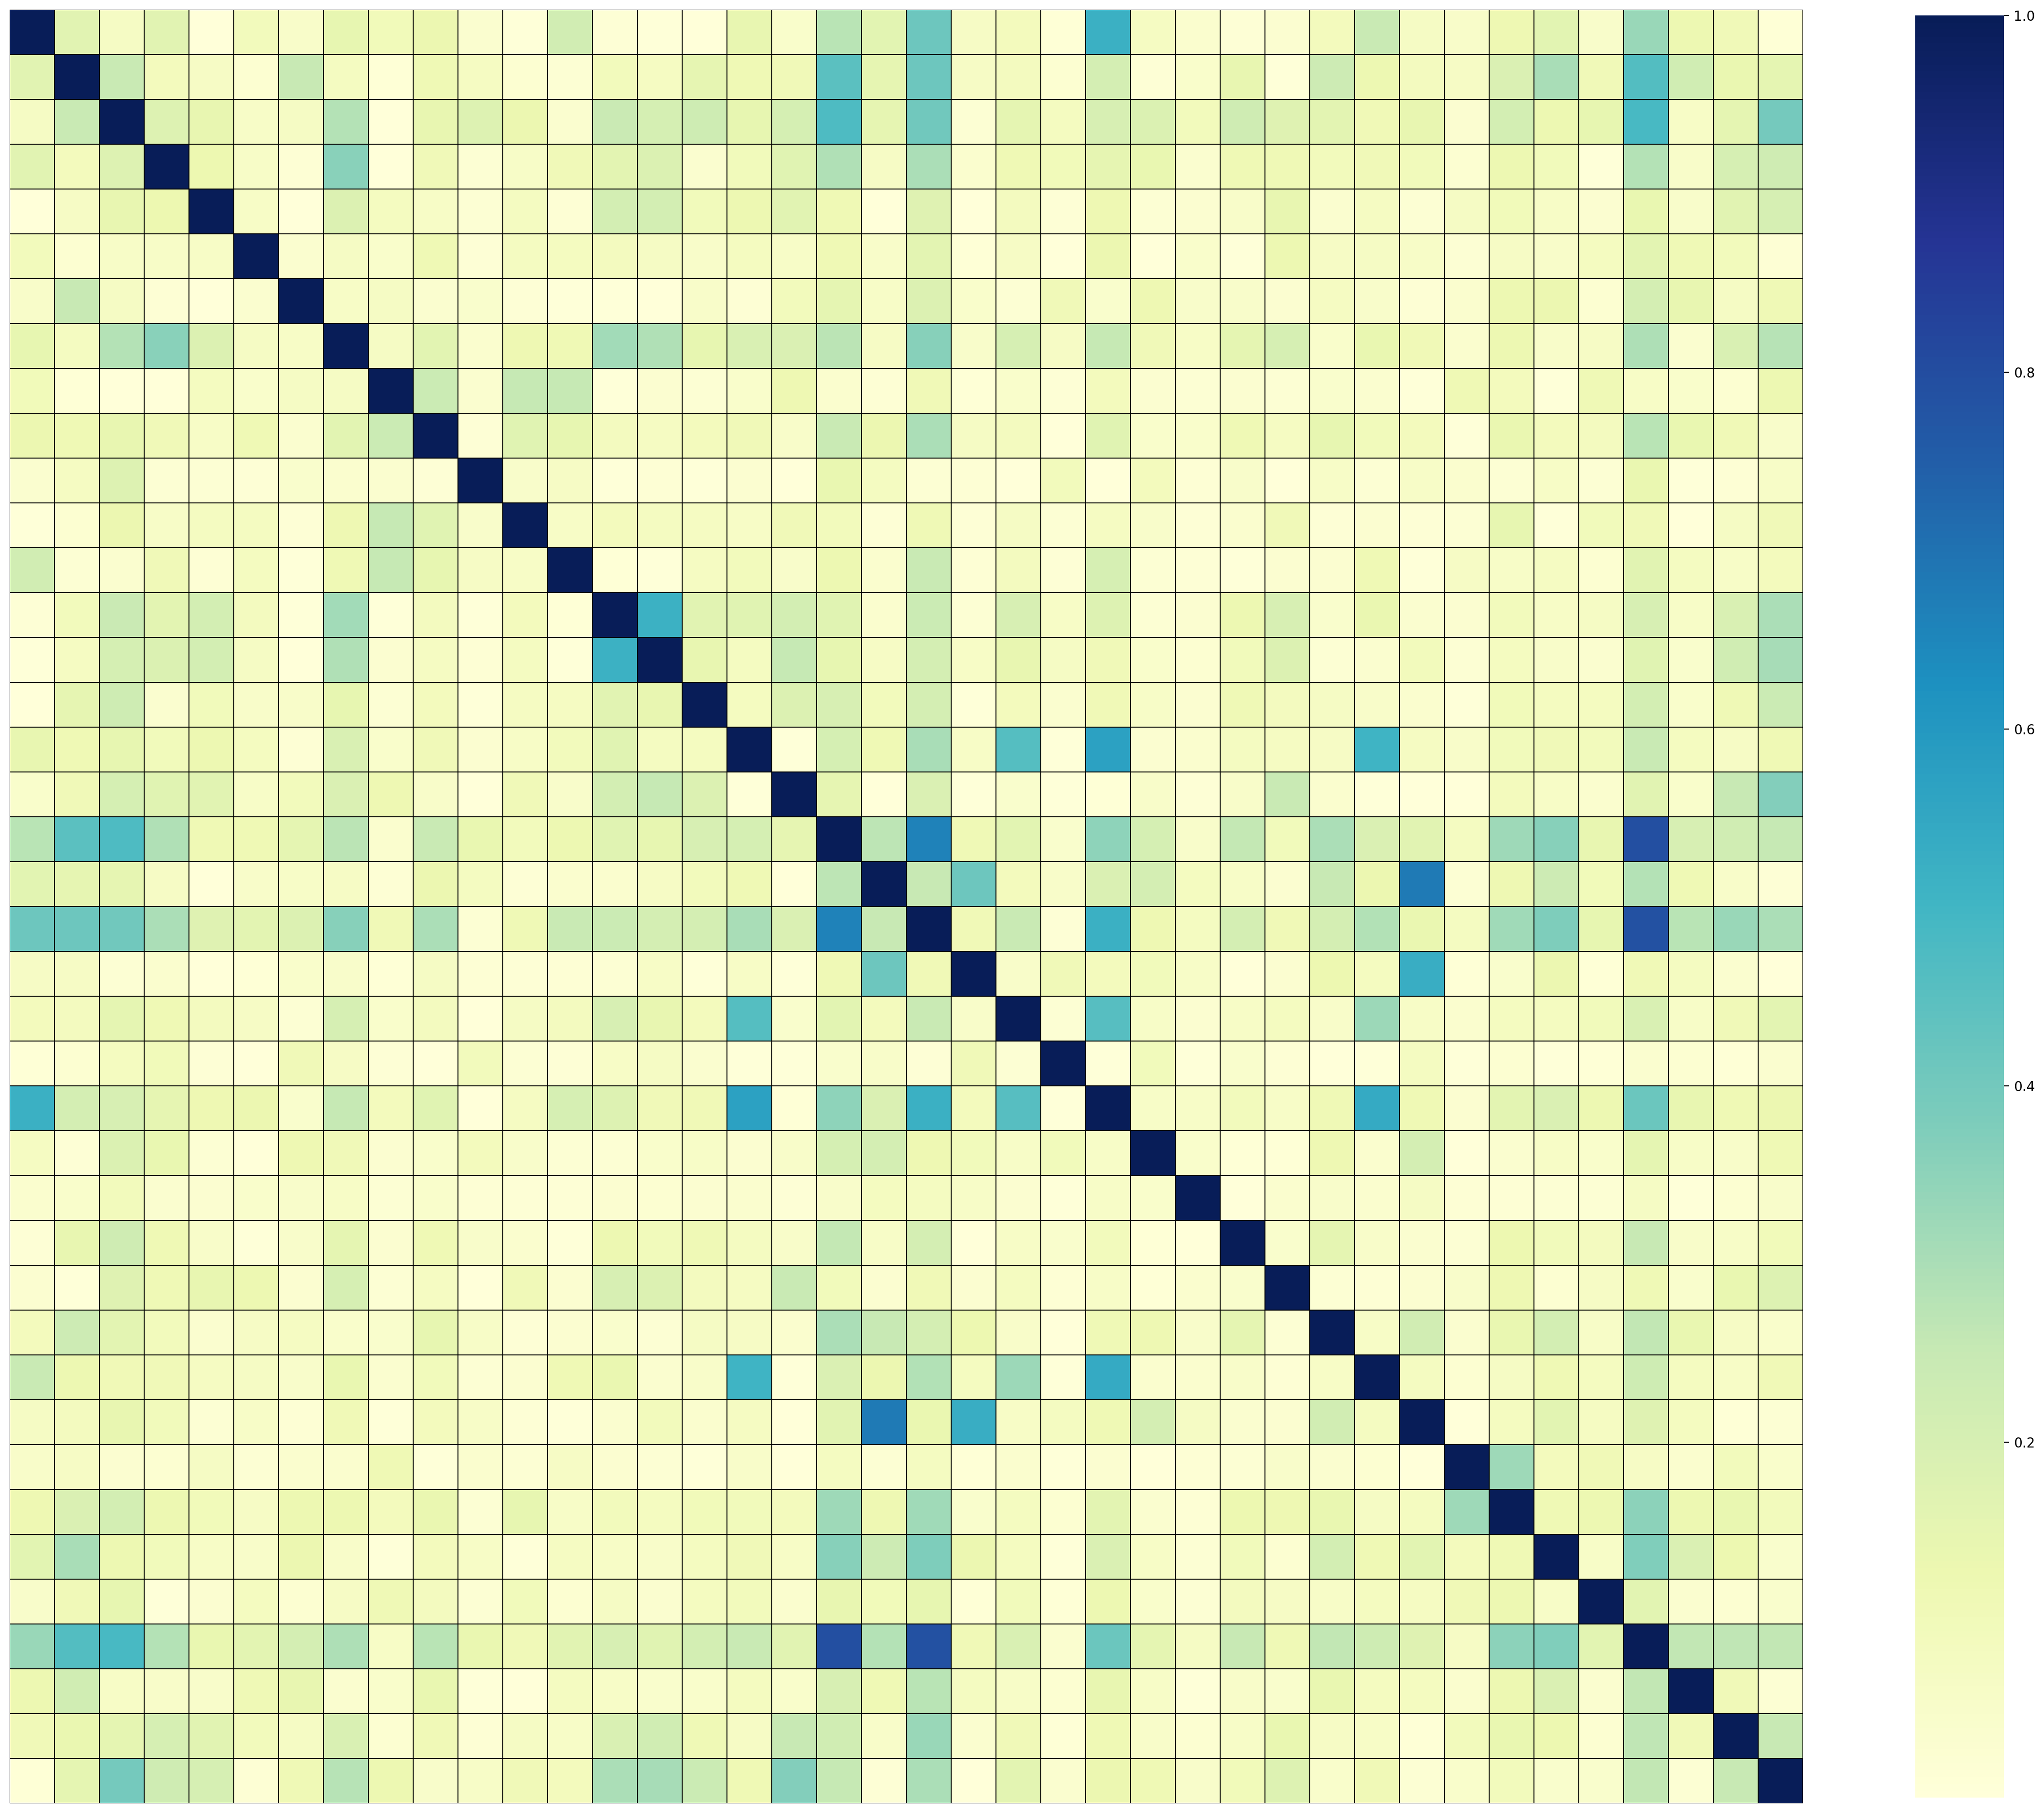
\includegraphics[width=0.3\textwidth]{figs/Spearman_noise_0.png}
%     %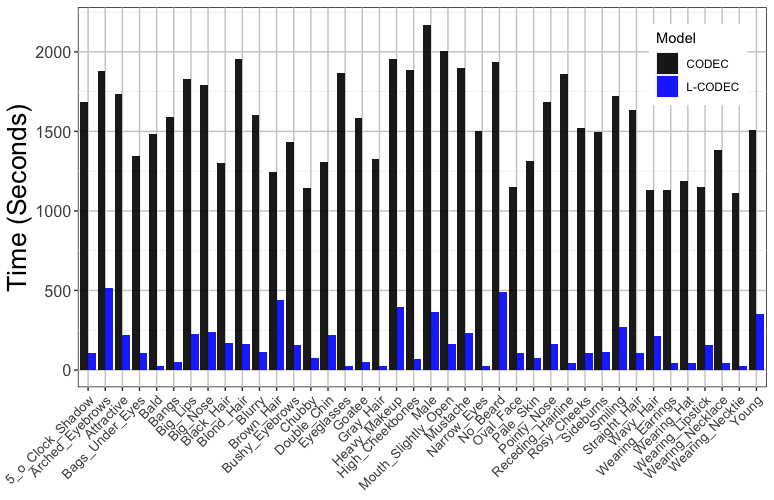
\includegraphics[width=0.45\textwidth]{figs/speed_hist.png}
%     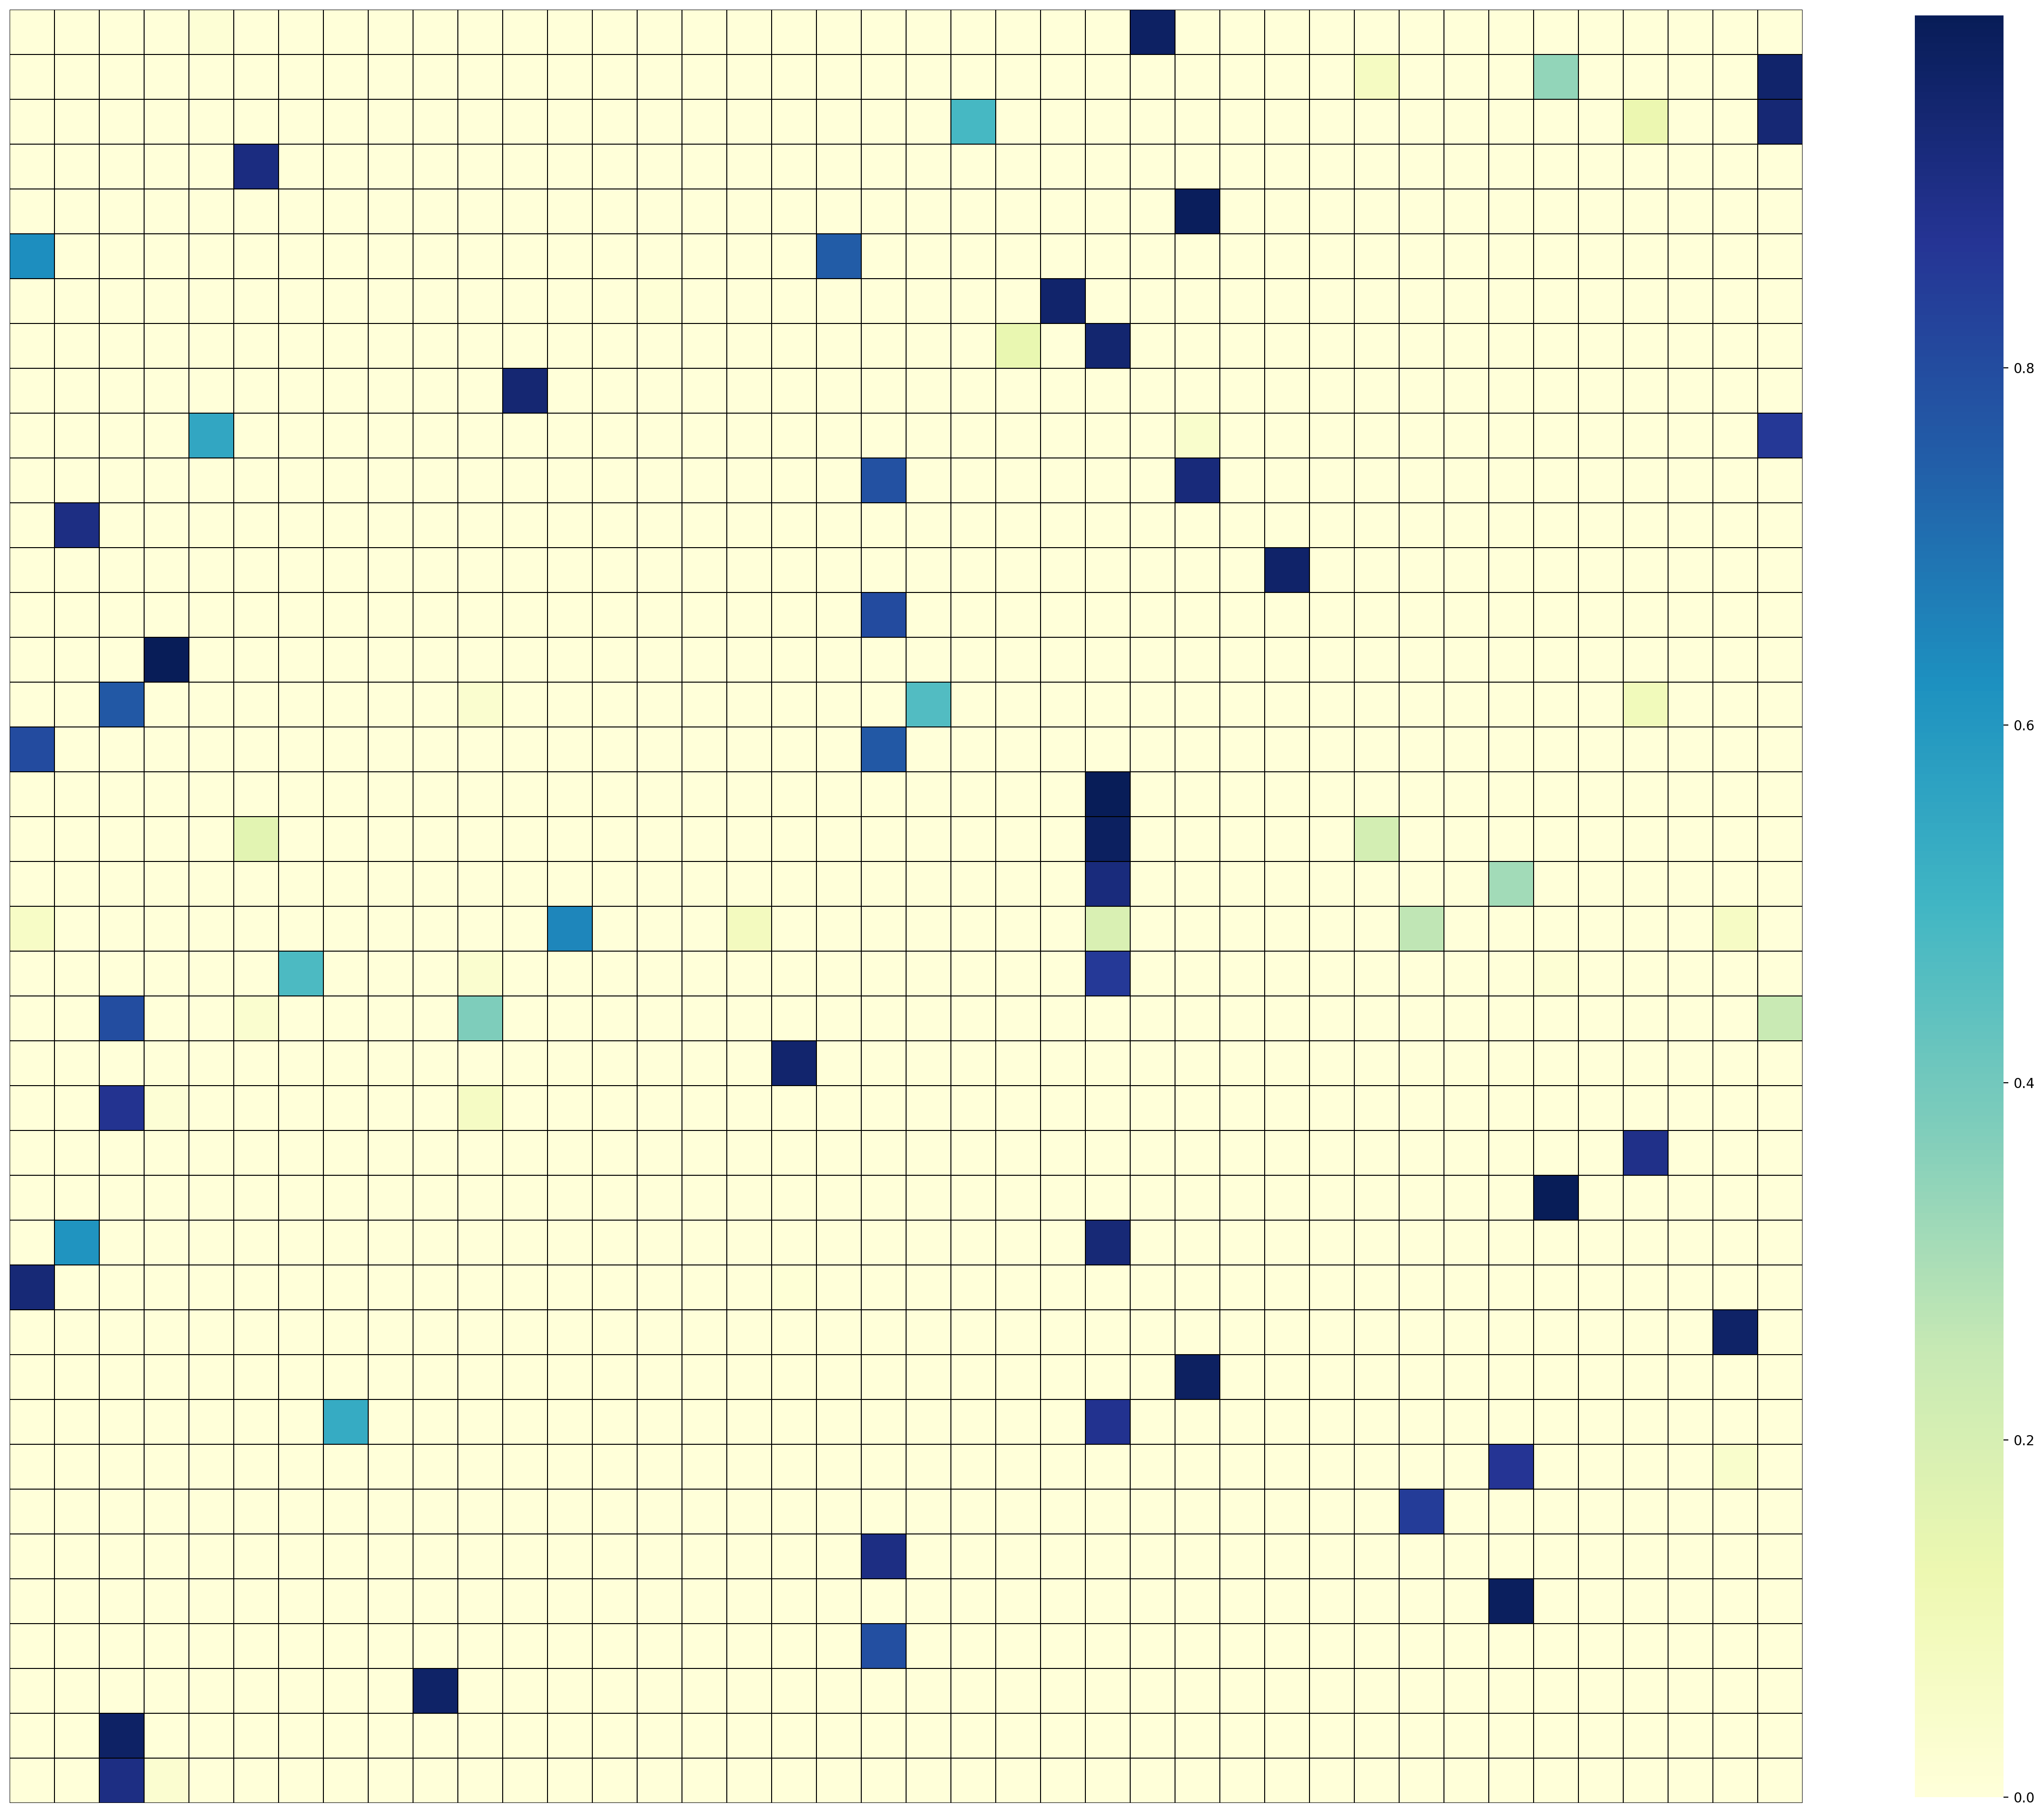
\includegraphics[width=0.3\textwidth]{figs/CODEC_noise_0.png}
%     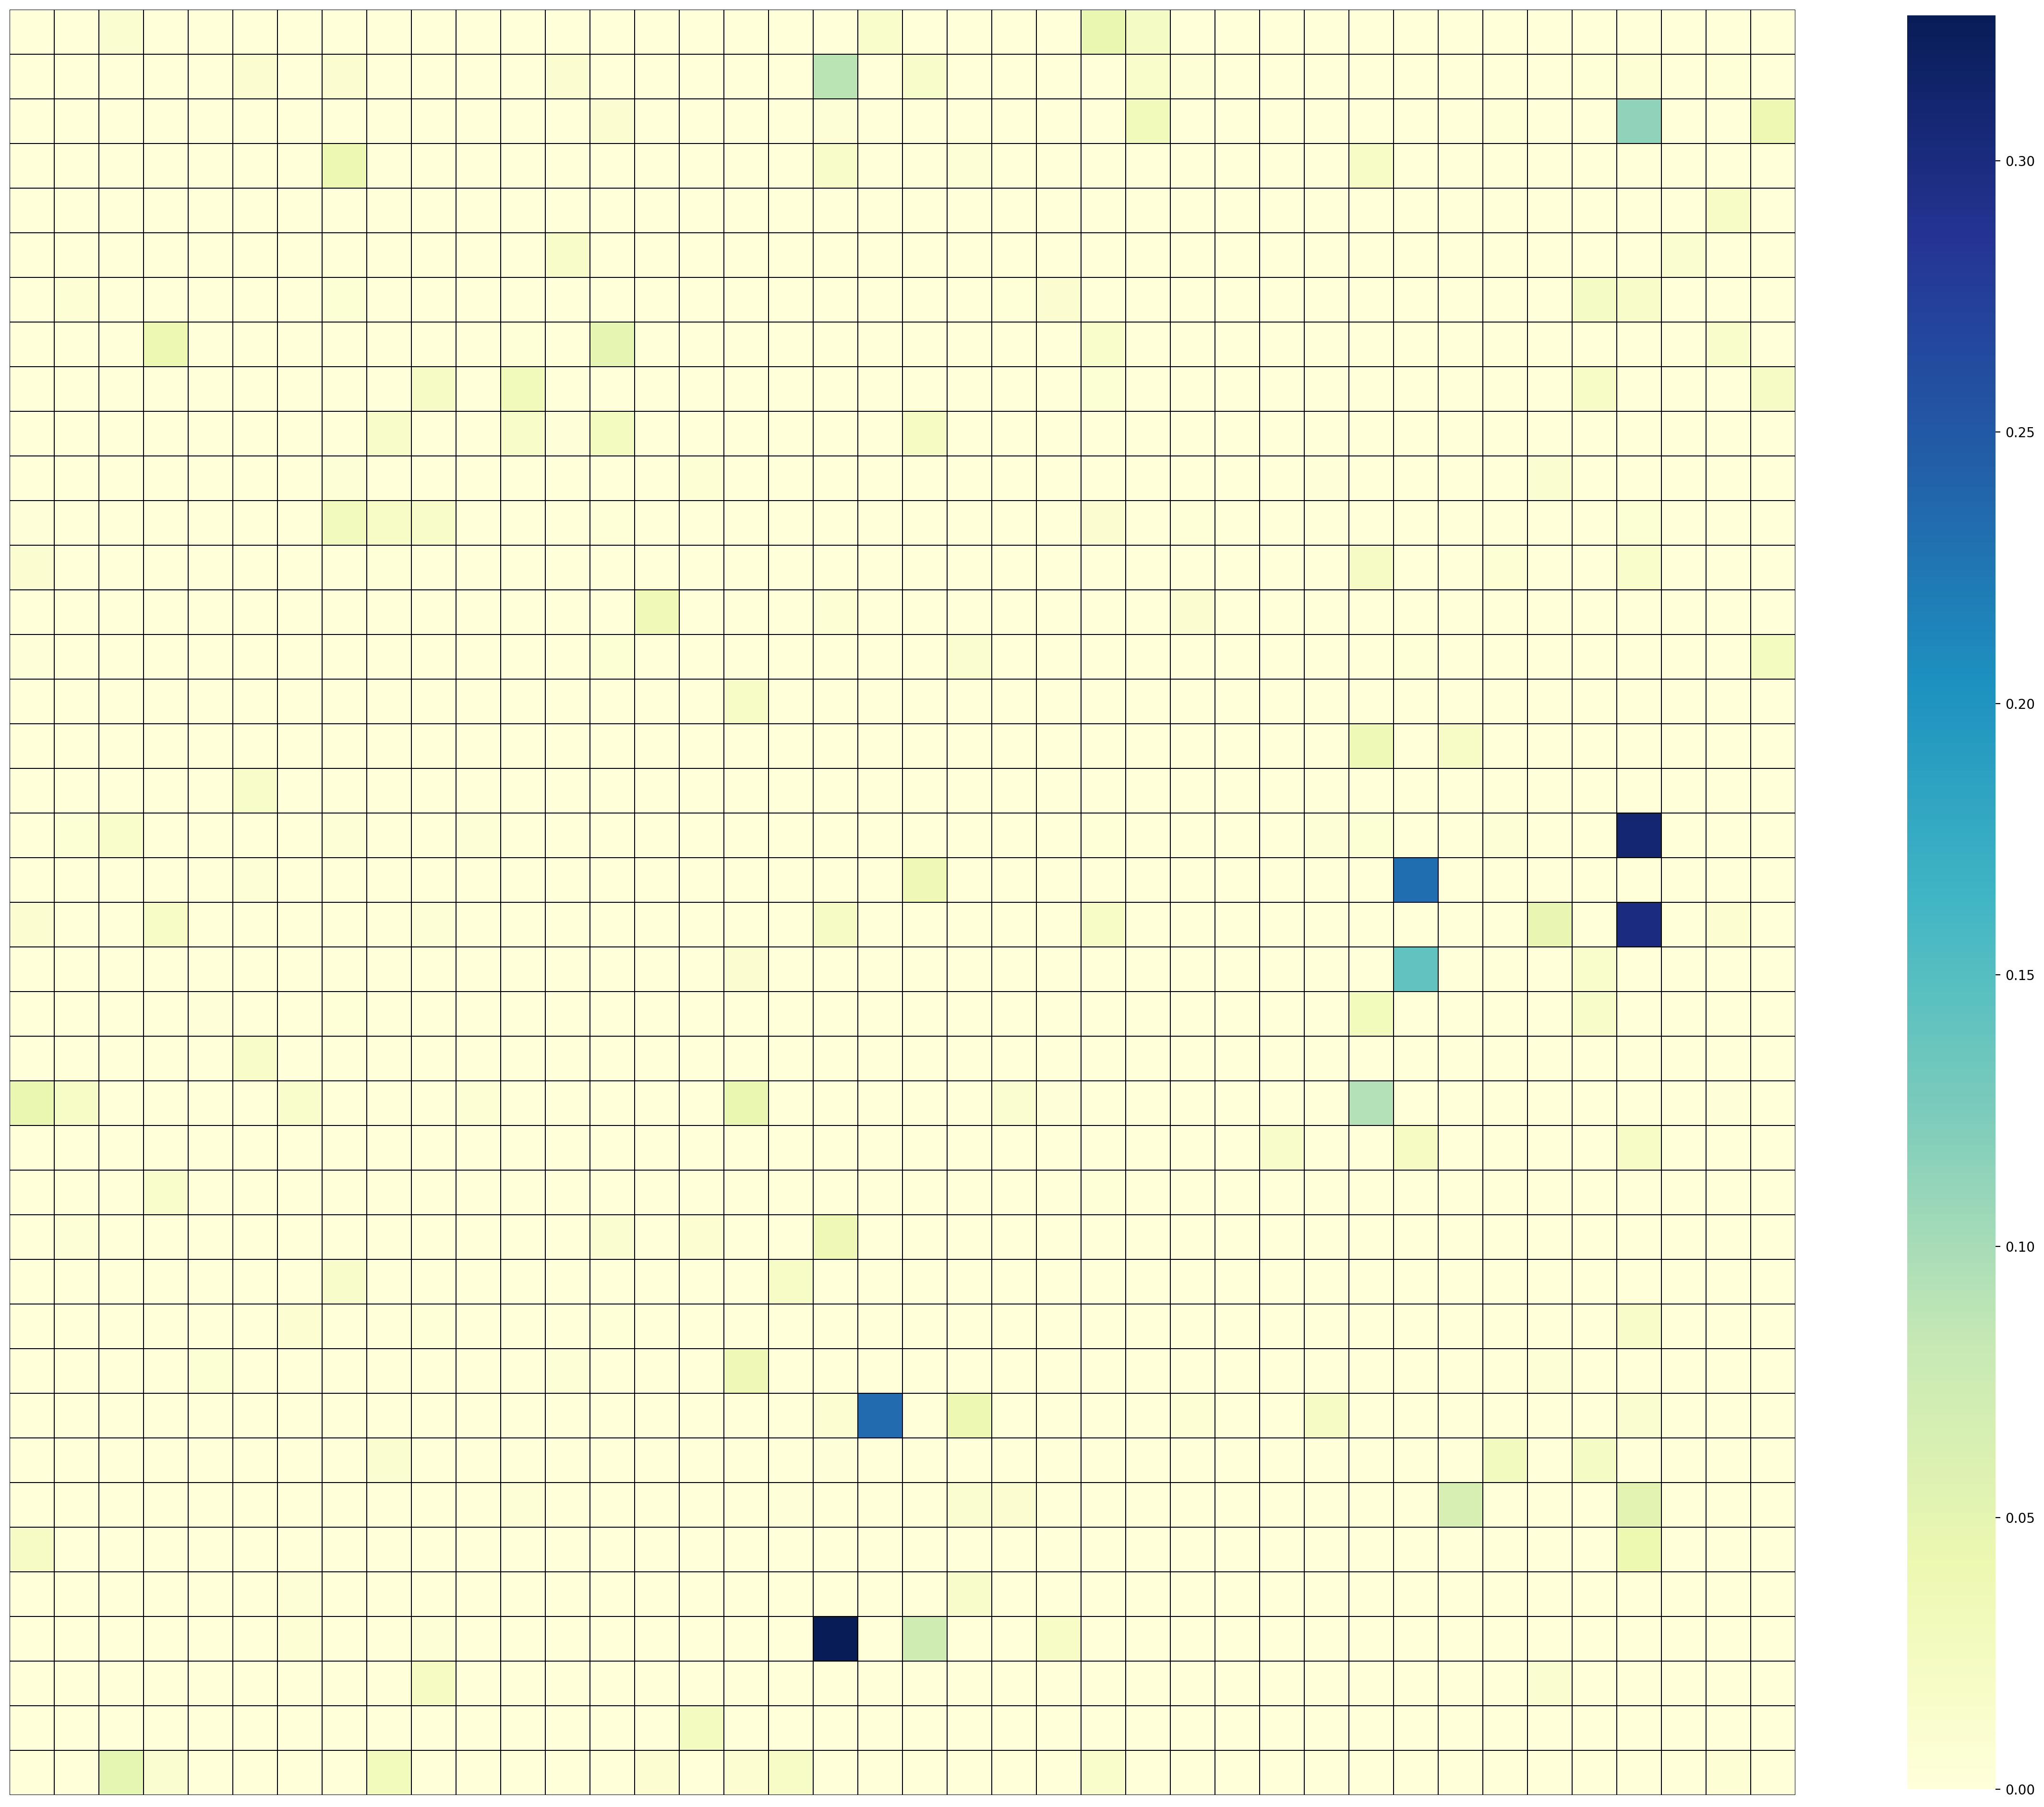
\includegraphics[width=0.3\textwidth]{figs/CODEC_noise_0.01.png}
%     \caption{Correlation matrices over the attributes in CelebA using (left) Spearman rank correlation, (middle) FOCI with CODEC, and (right) L-FOCI with  L-CODEC.}
%     \label{fig:corrmats}
% \end{figure}
\paragraph{L-CODEC Evaluation.}
To assess speedup gained in the discrete setting when running L-CODEC,
% We first demonstrate the additional speedup gained in the discrete setting when running L-CODEC.
we construct the Markov Blanket for specific attributes provided as side information with the CelebA dataset. Fig.~\ref{fig:speed_hist} shows the wall-clock times for Markov Blanket Selection via FOCI and L-FOCI for each attribute.
%{\color{red}In experiments, we use L-CODEC where discrete values or tiebreaks are common, and traditional CODEC when values are continuous or unique.}

\paragraph{Markov Blanket Identification.} We replicate the experimental setup in Sec 5.3 of \cite{bullseye}, where a high dimensional distribution over a ground truth graph is generated, and feature mappings are used to reduce the dimension and map to a latent space. Table~\ref{tab:bullseye} summarizes subset identification efficacy and runtime. Replacing conditional mutual information (CMI) with L-CODEC, we see a clear improvement in both runtime and Markov Blanket identification over the raw data, and comparable results in the latent feature space. Using L-FOCI directly in the feature space, we identify an additional spurious feature not part of the Markov Blanket, but runtime is significantly faster.
\begin{table}
    \centering
    \resizebox{!}{45pt}{%
    \begin{tabular}[b]{l|ccr|ccr}
        \hline\hline
        & \multicolumn{3}{c|}{Raw Data} & \multicolumn{3}{c}{Feature Maps} \\
        Method & TPR & FPR & Time (s) & TPR & FPR & Time (s) \\
        \hline
        \cite{bullseye} & 0.75 & 0.50 & 5124.22 & \textbf{0.875} & \textbf{0.00} & 516.19 \\
        L-CODEC + CIT & \textbf{1.00} & \textbf{0.50} & \textbf{402.10} & 0.75 & \textbf{0.00} & 117.29 \\
        L-CODEC + L-FOCI & \multicolumn{3}{c|}{N/A} & 0.833 & 0.50 & \textbf{0.464} \\
        \hline\hline
        % & \multicolumn{3}{c}{Feature Maps} \\
        % & TPR & FPR & Time (s) \\
        % \hline
        % \cite{bullseye}  & \textbf{0.875} & \textbf{0.00} & 516.19 \\
        % L-CODEC + CIT & 0.75 & \textbf{0.00} & 117.29  \\
        % L-CODEC + L-FOCI & 0.833 & 0.50 & \textbf{0.464} \\
        % \hline\hline
    \end{tabular}
    %
    }
    \caption{\label{tab:bullseye} 3D-Bullseye Markov Blanket identification. CIT represents the model in \cite{bullseye}. Both L-CODEC and L-FOCI run much faster than recent Markov Blanket identification schemes. L-FOCI is not applicable to the multi-dimensional raw data setting.}
\end{table}
% \begin{table}
% \centering
% \begin{tabular}{l|cccccc}
%     \hline\hline
%     & \multicolumn{3}{c}{Raw Data} & \multicolumn{3}{c}{Feature Maps} \\
%     & TPR & FPR & Time (s) & TPR & FPR & Time (s) \\
%     \hline
%     CMI + CIT \cite{bullseye} & 0.75 & 0.50 & 5124.22  & \textbf{0.875} & \textbf{0.00} & 516.19 \\
%     L-CODEC + CIT & \textbf{1.00} & \textbf{0.50} & \textbf{402.10} & 0.75 & \textbf{0.00} & 117.29  \\
%     L-CODEC + L-FOCI & -- & -- & -- & 0.833 & 0.50 & \textbf{0.464} \\
%     \hline\hline
% \end{tabular}
% \begin{tabular}{l|ccc}
%     \hline\hline
%     & \multicolumn{3}{c}{Raw Data} \\
%     & TPR & FPR & Time (s) \\
%     \hline
%     CMI + CIT \cite{bullseye} & 0.75 & 0.50 & 5124.22 \\
%     L-CODEC + CIT & \textbf{1.00} & \textbf{0.50} & \textbf{402.10} \\
%     L-CODEC + L-FOCI & -- & -- & -- \\
%     \hline\hline
% \end{tabular}
% \begin{tabular}{l|ccc}
%     \hline\hline
%     & \multicolumn{3}{c}{Feature Maps} \\
%     & TPR & FPR & Time (s) \\
%     \hline
%     CMI + CIT \cite{bullseye}  & \textbf{0.875} & \textbf{0.00} & 516.19 \\
%     L-CODEC + CIT & 0.75 & \textbf{0.00} & 117.29  \\
%     L-CODEC + L-FOCI & 0.833 & 0.50 & \textbf{0.464} \\
%     \hline\hline
% \end{tabular}
% \caption{\label{tab:bullseye} 3D-Bullseye Markov Blanket identification. CIT represents the conditional independence testing framework used in \cite{bullseye}. Both L-CODEC and L-FOCI run significantly faster then recent Markov Blanket identification schemes.}
% \end{table}

% Setup 2 (Complex Dependencies): previous is somewhat ``proprotional". Describe DAG from random base operations (Ronak's synthetic. Same eval as above.



% In this set of experiments, we take advantage of the selective power of conditional independence scores to identify a set of spurious features. We think of spurious features as ones that can maliciously influence the decision making process of the models being learned by virtue of their non-trivial correlation with the target attribute. In the experiments presented in this paper, we consider the CelebA dataset and consider the task of binary classification for certain attributes which we decide based on our observations of spurious features. 
% We consider the prediction of attributes: ``Wearing Lipstick", ``Young", ``No Beard" and ``Smiling" in four different experiments. 
% The key step is to identify the spurious features for each of these attributes separately.
% For that, we use the L-CODEC algorithm described above with varying amounts of noise. 
% Once the spurious attributes are identified, we use them in a Gradient Reversal framework for regularizing against the spurious attributes, while predicting the specific target attribute.
% The prediction model being considered in these experiments is the MobileNet-V2. We use this architecture for a 2-class prediction
% problem and train it from scratch. The experimental results are presented in the table and discussed below.
% When using the full set of attributes, we significantly reduce performance, even with a number of different parameter settings.
% Unregularized, we can clearly see a biased model with respect to the attributes of interest.



%\begin{outline}[enumerate]
%\1 describe synthetic graph setup
%    \2 describe results
%    \2 immediate identification of markov blanket
%\1 describe bullseye setup (2d/3d)
%    \2 replacing statistic
%    \2 replacing entire procedure
%    \2 describe results
%    \2 significantly faster with similar results
%\1 What can we do with it? CelebA
%    \2 identify markov blanket over specific attribute vs others
%    \2 add invariance via gradient reversal
%    \2 compare performance on full set and conditioned set when small set and full set of features is conditioned
%        \3 full set is too bad, drastic drop in acc
%        \3 select only spurious features
%\end{outline}

% \input{_explain.tex}

\begin{figure}[t]
    \centering
    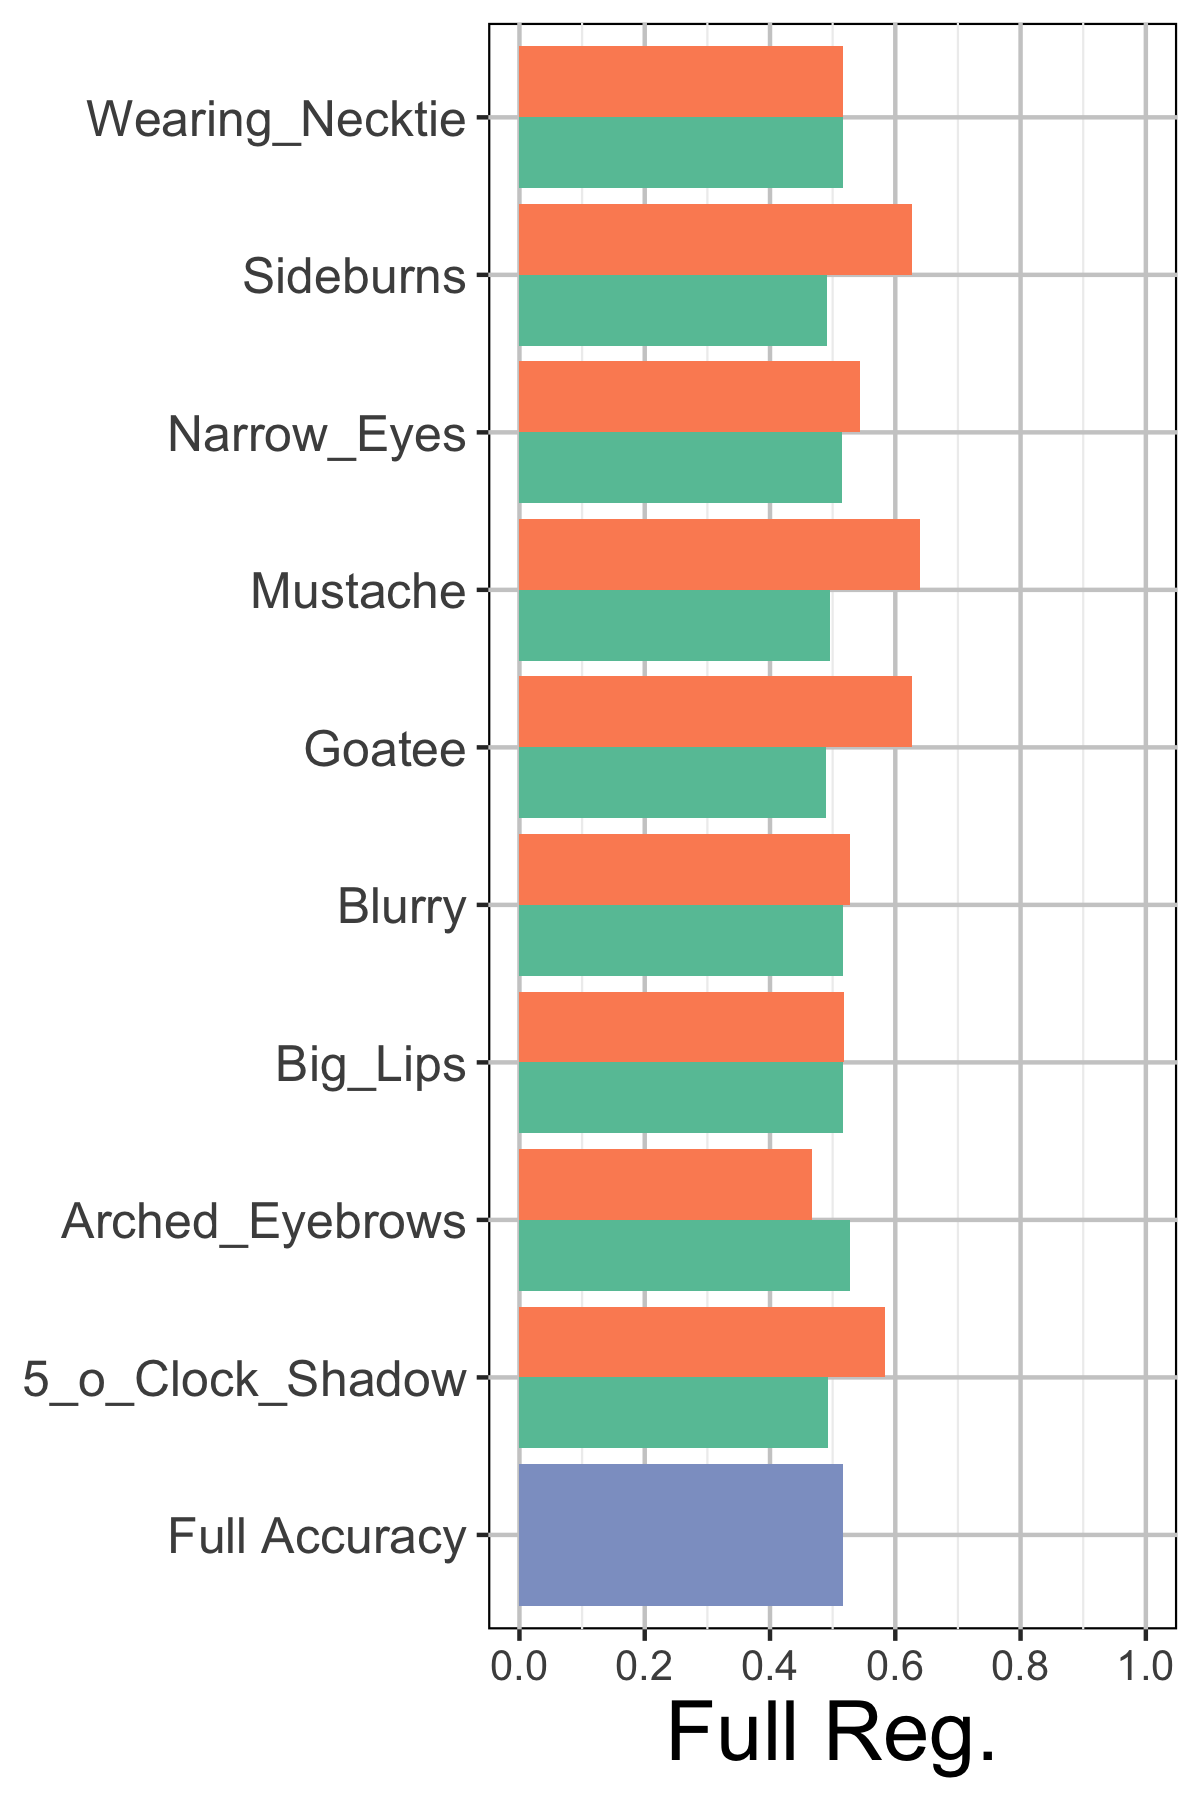
\includegraphics[width=0.155\columnwidth,trim={0.25in 0 10.25in 0},clip]{5_unlearn/figs/No_Beard_All.png}
    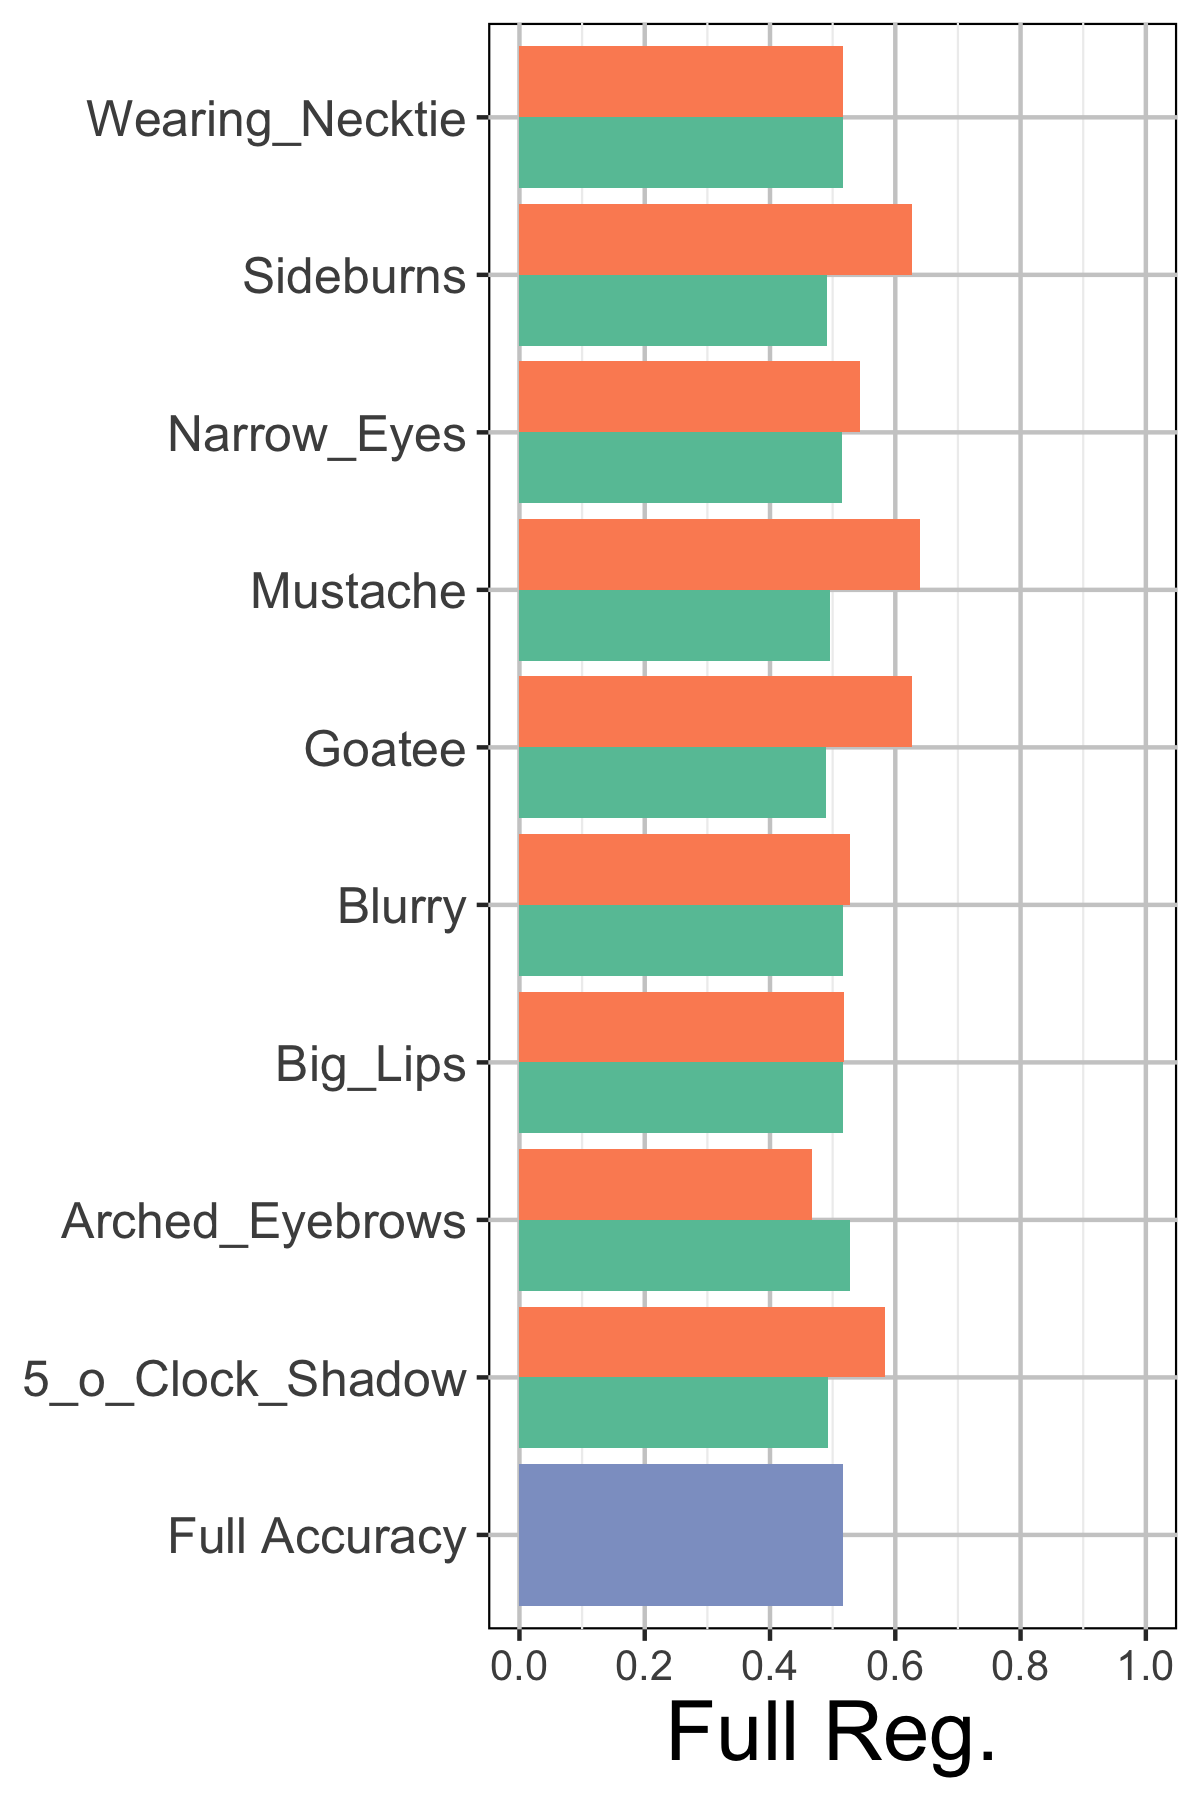
\includegraphics[width=0.25\columnwidth,trim={6.5in 0 0 0},clip]{5_unlearn/figs/No_Beard_All.png}
    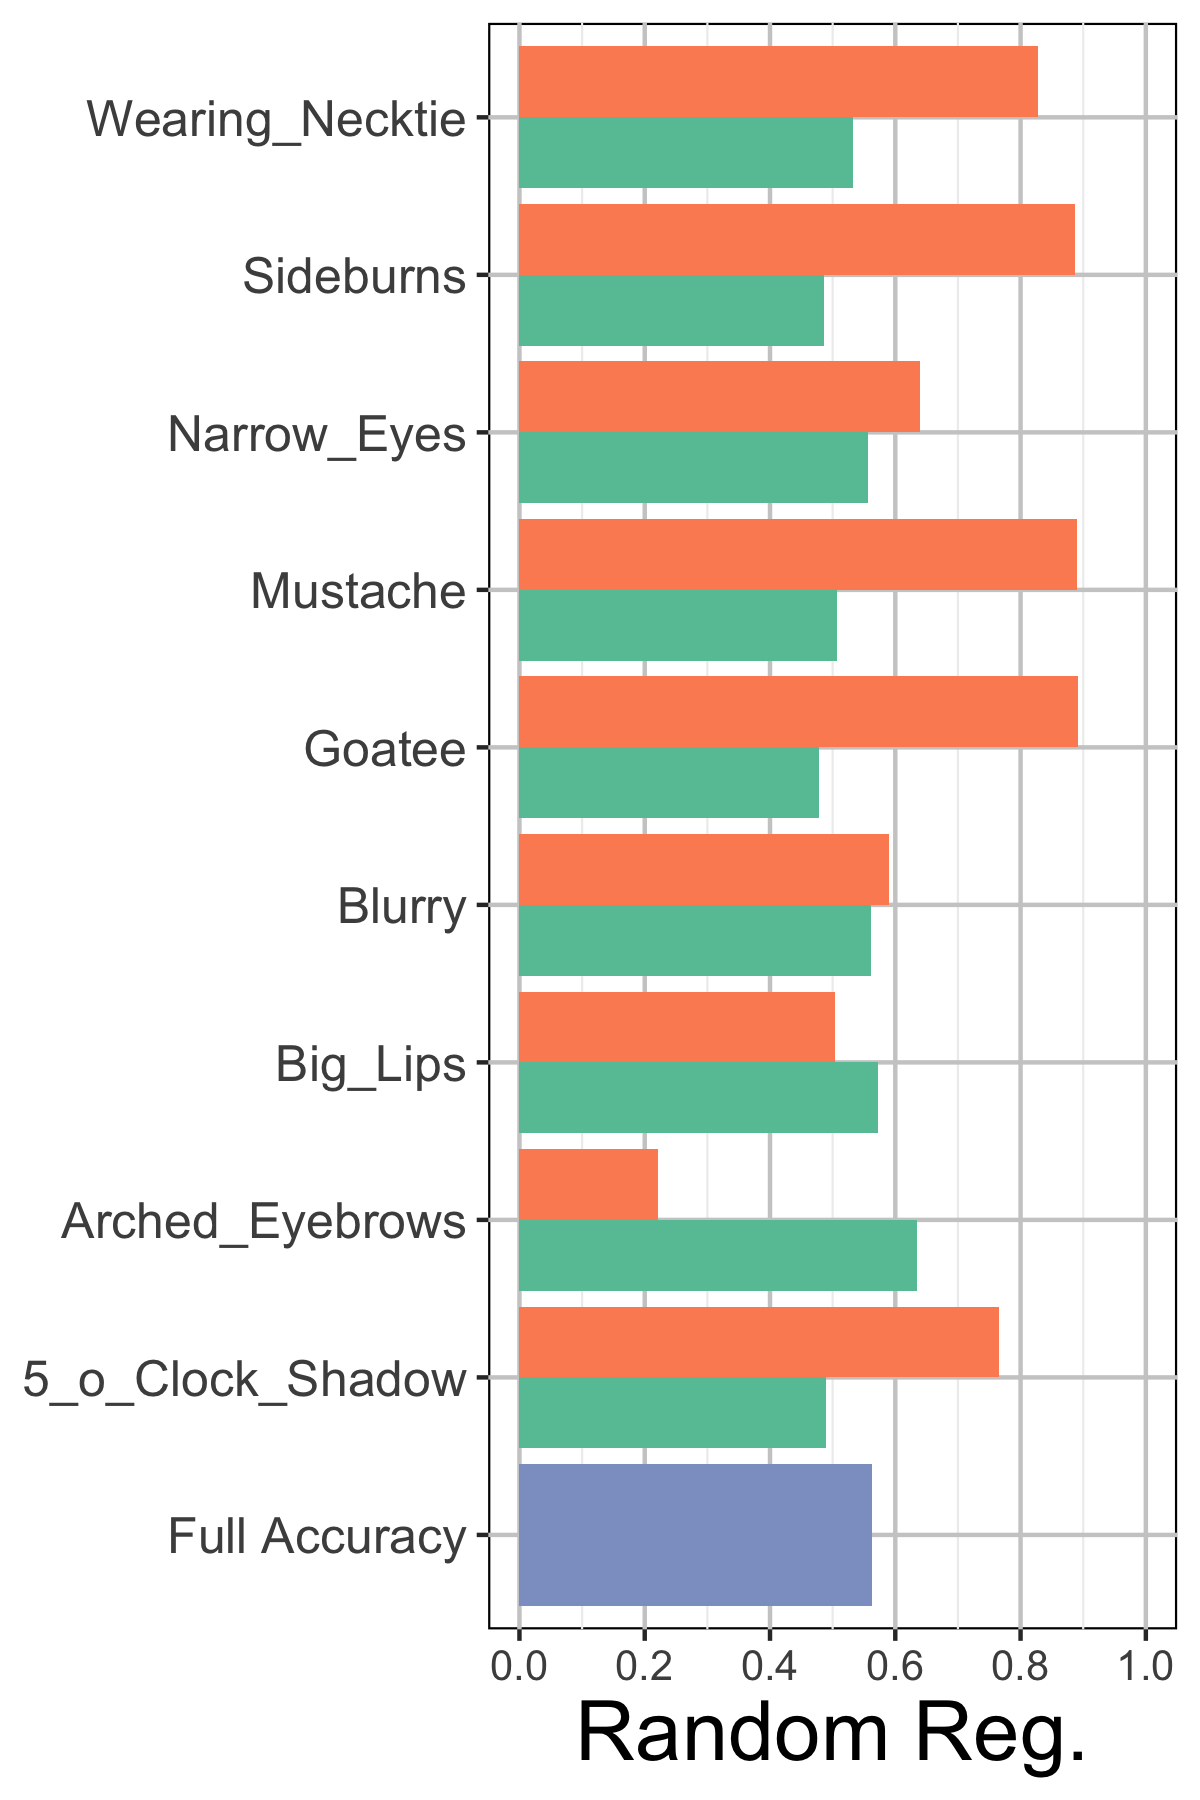
\includegraphics[width=0.25\columnwidth,trim={6.5in 0 0 0},clip]{5_unlearn/figs/No_Beard_Random.png}
    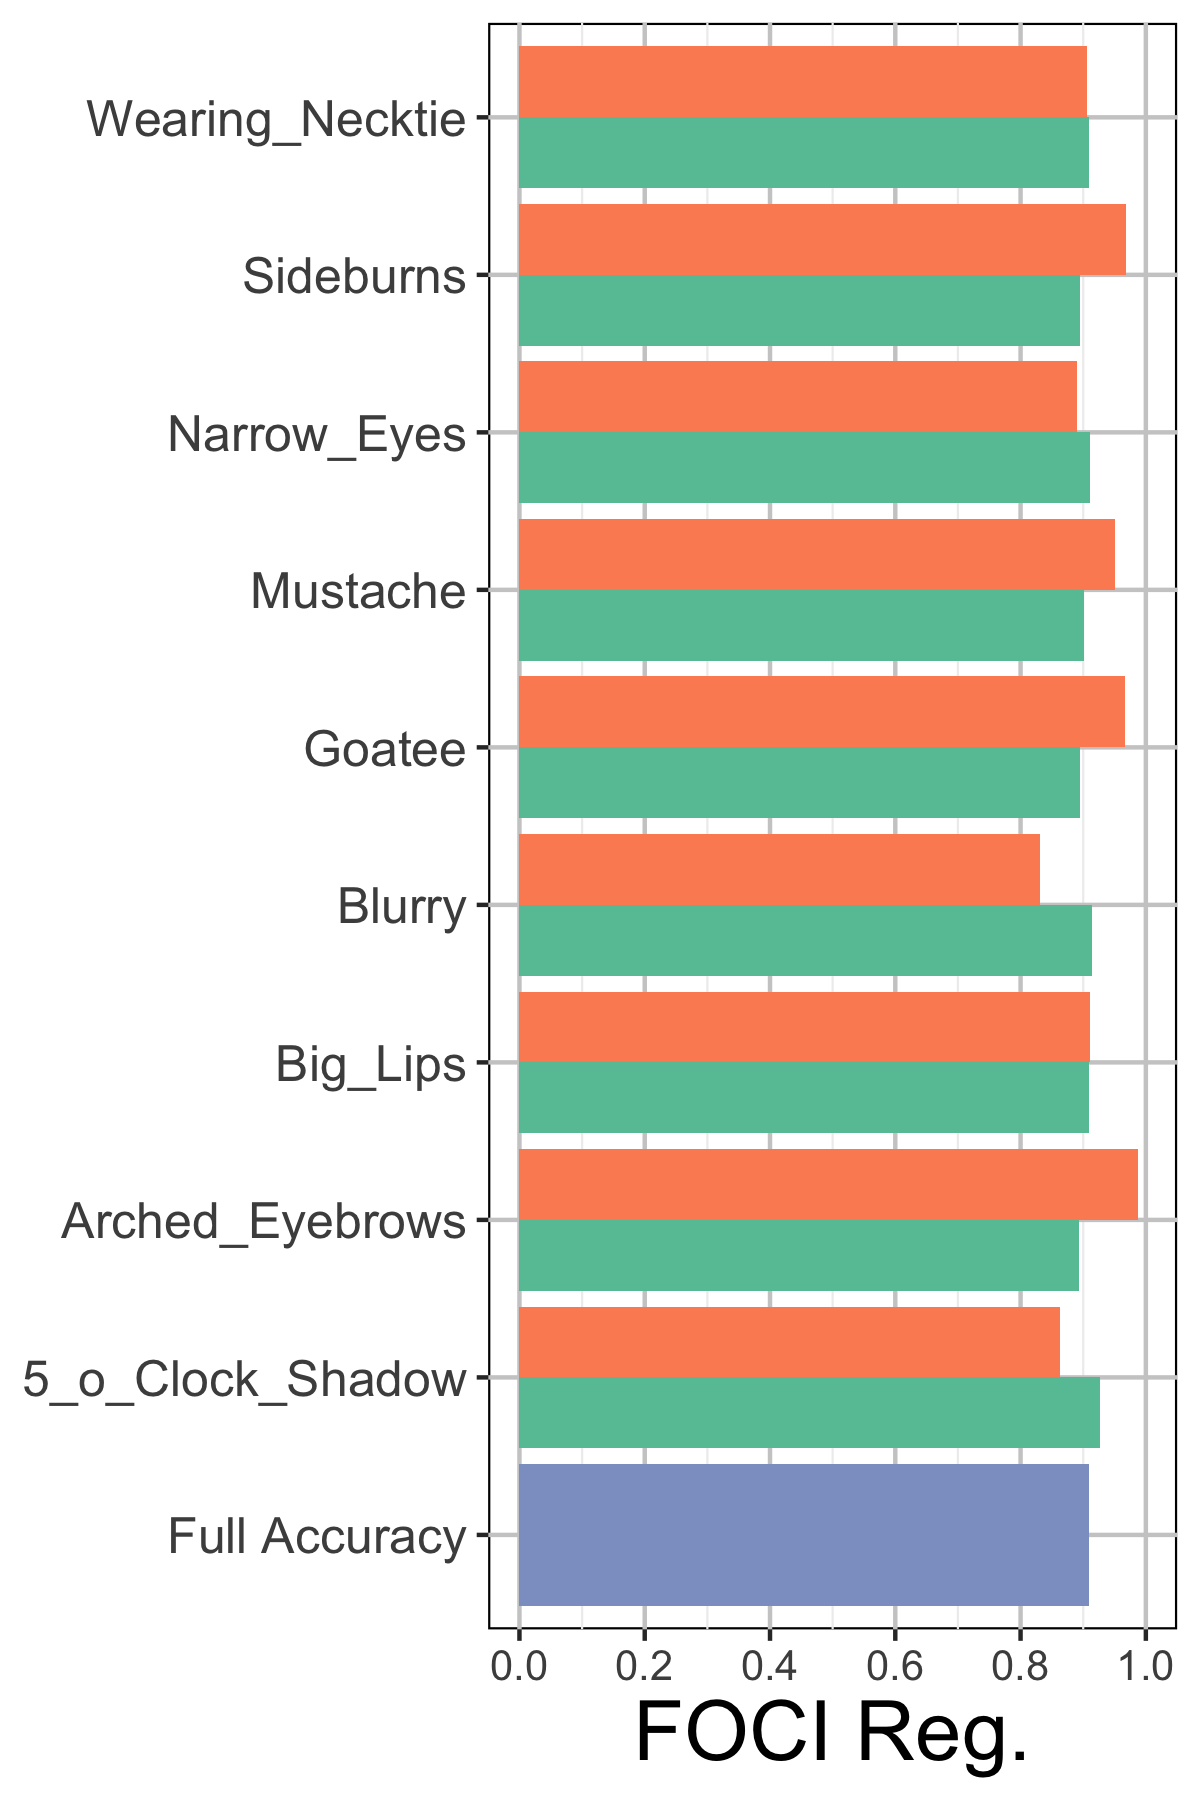
\includegraphics[width=0.25\columnwidth,trim={6.5in 0 0 0},clip]{5_unlearn/figs/No_Beard_FOCI.png}
    \vspace{-8pt}
    \caption{\label{fig:spur} Validation accuracies after training to predict ``No Beard" in the CelebA dataset. (L to R) regularization for all features, for a random subset, and via FOCI. Green indicates accuracy on the data with that feature, red, without.}
    \vspace{-15pt}
\end{figure}

\paragraph{Spurious Feature Regularization.}
This Markov Blanket $(MB)$ identification scheme can be used to address spurious feature effects on traditional NN models.
%In modern machine learning applications, strict classification or regression on outcomes of interest is no longer sufficient to deploy models in the real world. 
%Particularly, a large number of existing machine learning problems such as overfitting to spurious features and class imbalance can drastically affect model performance on biased training data. 
% Removing the effect of spurious features can be achieved in many ways, but it requires knowledge of which features should be considered.
% Here, we look at applications in which there may be a large number of outside factors, or side information, that may be heavily dependent, or spurious, to the outcome variable. 
%Using typical tools in the ML toolbox,
% A natural method of attempting to incorporate side information would be to add appropriate loss terms to the global objective, where the loss terms may be pushing the learning algorithm towards \textit{regularized} models that are further away from the training set optimum, but closer to the solution of the true question.
A straightforward approach would be to directly add a loss term for each potentially important feature over which we would like to regularize, 
$\cL(\theta) + \sum_{S\in \cS} R_S(\theta)$.
However, with a large number of outside factors $S$, this can adversely effect training.
% ,to the point where for any reasonable regularization parameter settings no model is able to be found with high performance on the outcome of interest. 
We instead use L-FOCI to identify the set of minimal factors that, when conditioned, make the rest conditionally independent. Then it is only necessary to include regularizers over $S \in MB(Y)$.
%Here, if we consider a graph over the external factors and our outcome of interest, it is immediately clear that if we wish to regularize the effect of all factors, it is sufficient to only regularize the effect of the Markov Blanket. 
% \begin{align}
% \cL(\theta) + \sum_{S\in MB(Y)} R_S(\theta)
% \end{align}

We evaluate a simple attribute image classification setting using the CelebA dataset. We run L-FOCI over the attributes as in our L-CODEC evaluation, and regularize using a Gradient Reversal Layer for a simple accuracy term over those attributes.
% We compare models with varying regularization over all attributes, randomly chosen attributes, and FOCI-selected attributes.
Results in Fig. \ref{fig:spur} clearly show that selection with FOCI provides the best result, maintaining high overall accuracy but also preserving high accuracy on sets of samples with/without correlated attributes.

\section{L-FOCI for Machine Unlearning}

\subsection{Compare to Full Hessian Computation}
For simple regressors, we can compute the full Hessian and compare results generated by a traditional unlearning update, our L-FOCI update, and a random selection update. To reduce variance and show the best possible random selection, we run our L-FOCI and randomly choose a set of the same size for each random selection. Fig.~\ref{fig:mnistcifar} (left) shows validation and residual accuracies for 1000 random removals from MNIST (average over 10 runs). 

\begin{figure*}[h!]
    \centering
    %\includegraphics[width=0.3\textwidth]{figs/scrub/MNIST_Valid_Acc.png}
    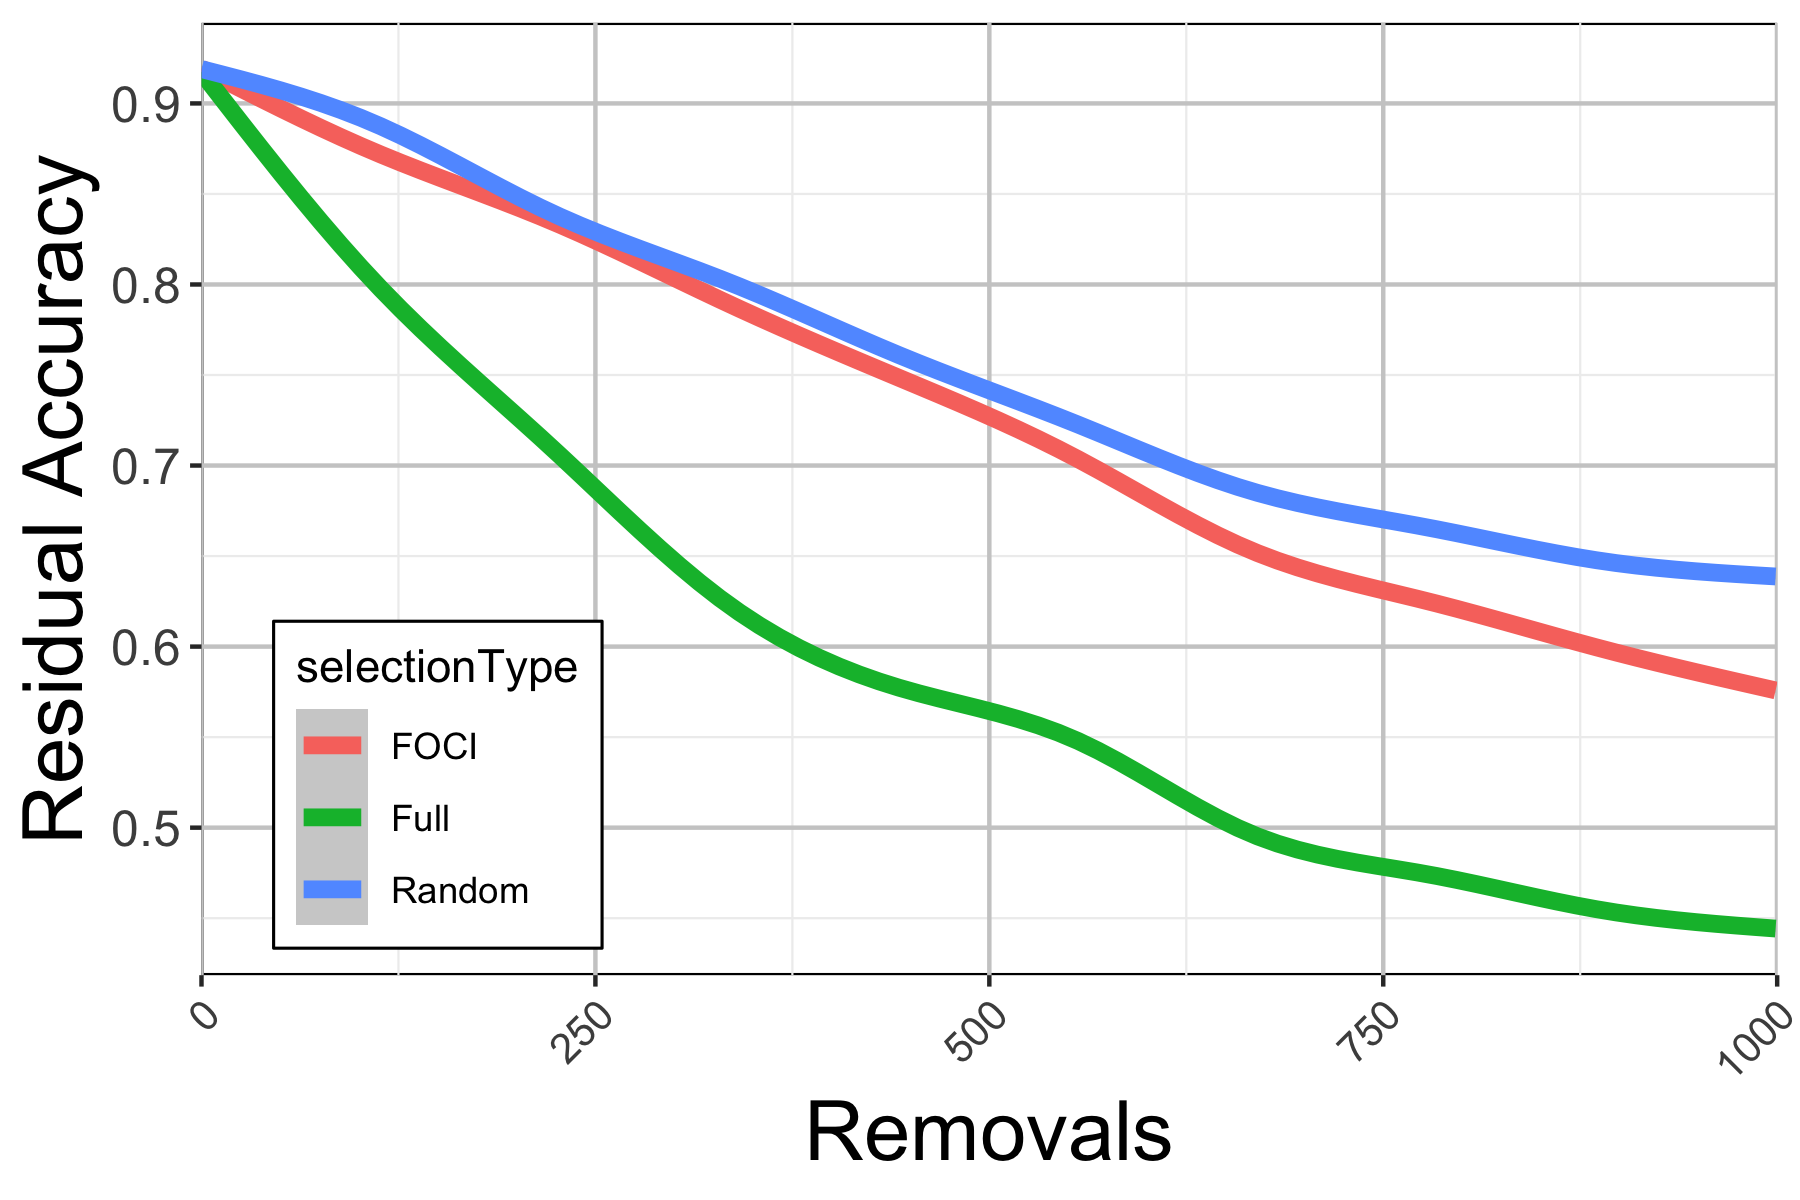
\includegraphics[width=0.24\textwidth]{5_unlearn/figs/scrub/MNIST_Resid_Acc.png}
     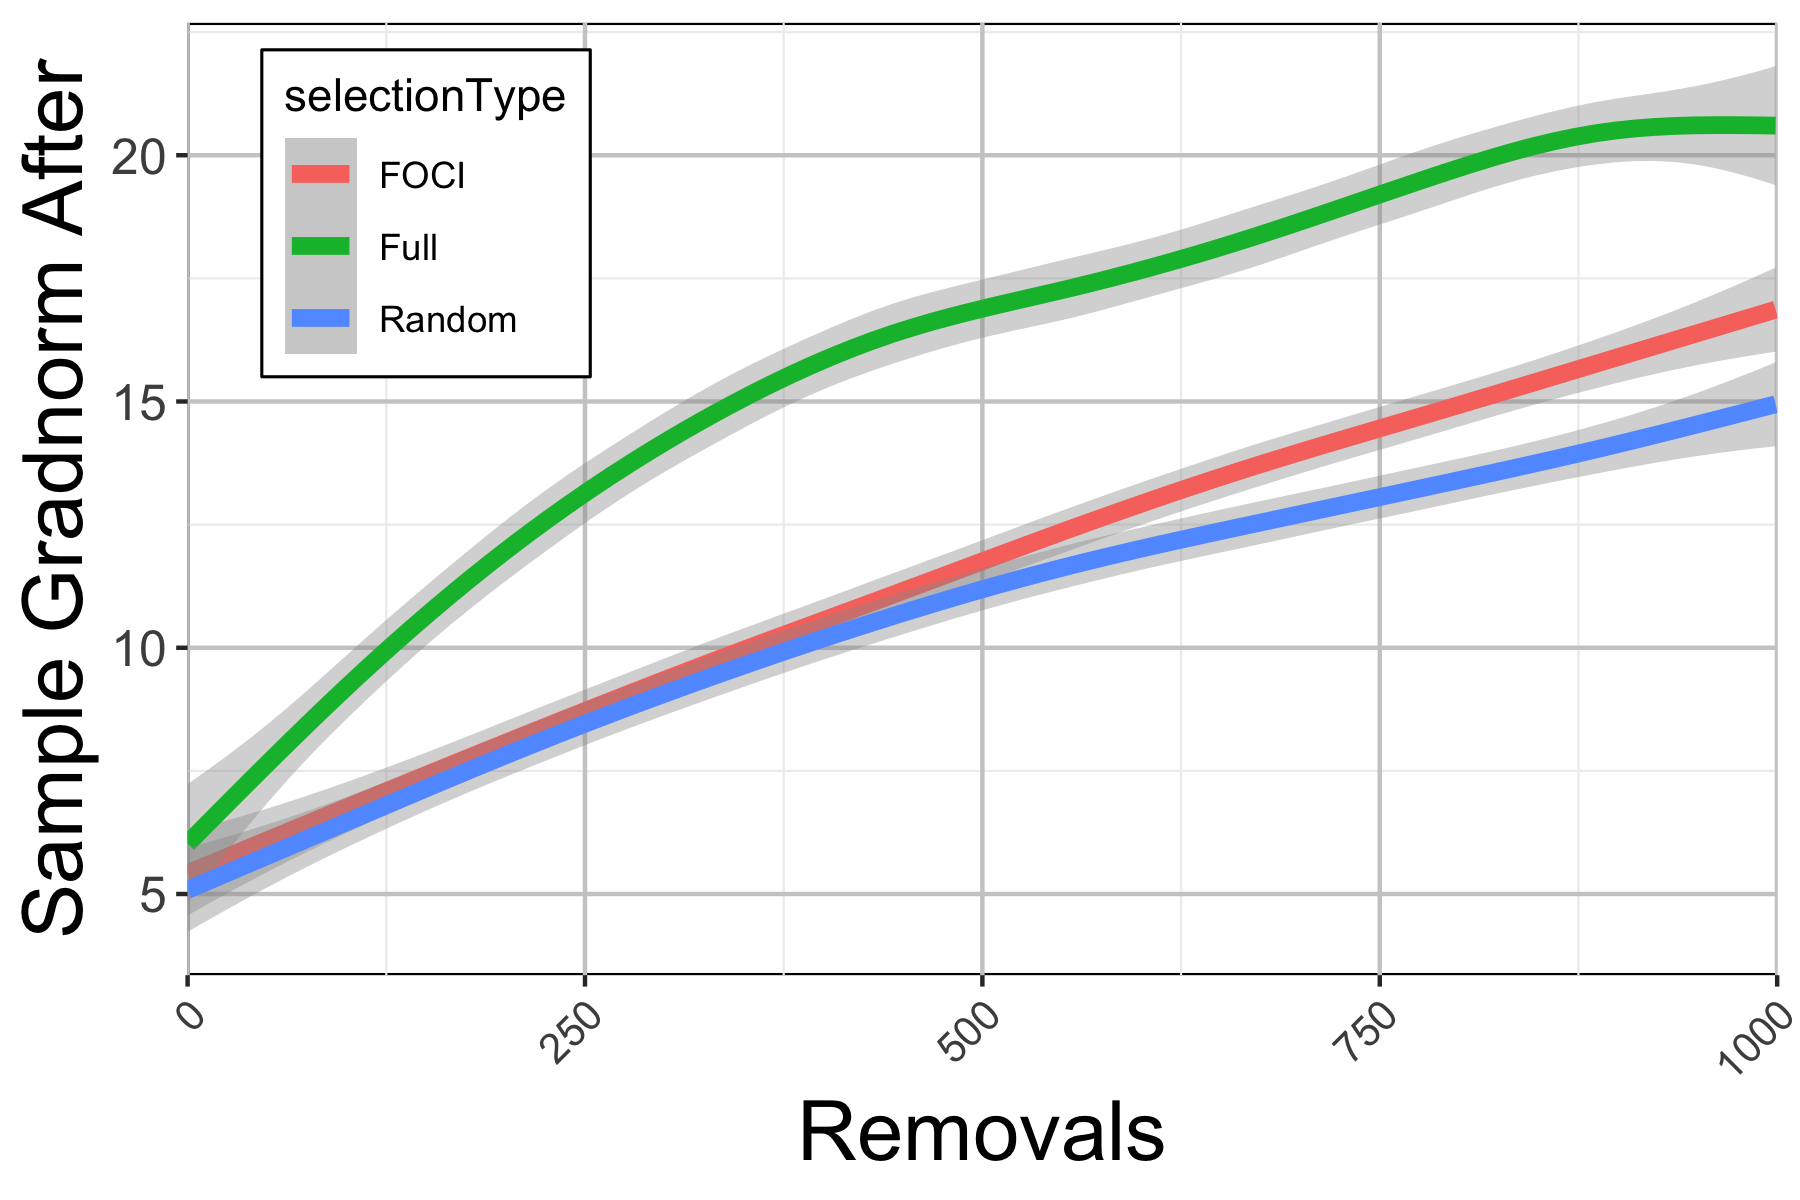
\includegraphics[width=0.24\textwidth]{5_unlearn/figs/scrub/MNIST_GradNorm_Logistic.png}
     \vspace{-8pt}
    % \label{fig:mnist}
    % \includegraphics[width=0.33\textwidth]{5_unlearn/figs/scrub/cifar_val.png}
    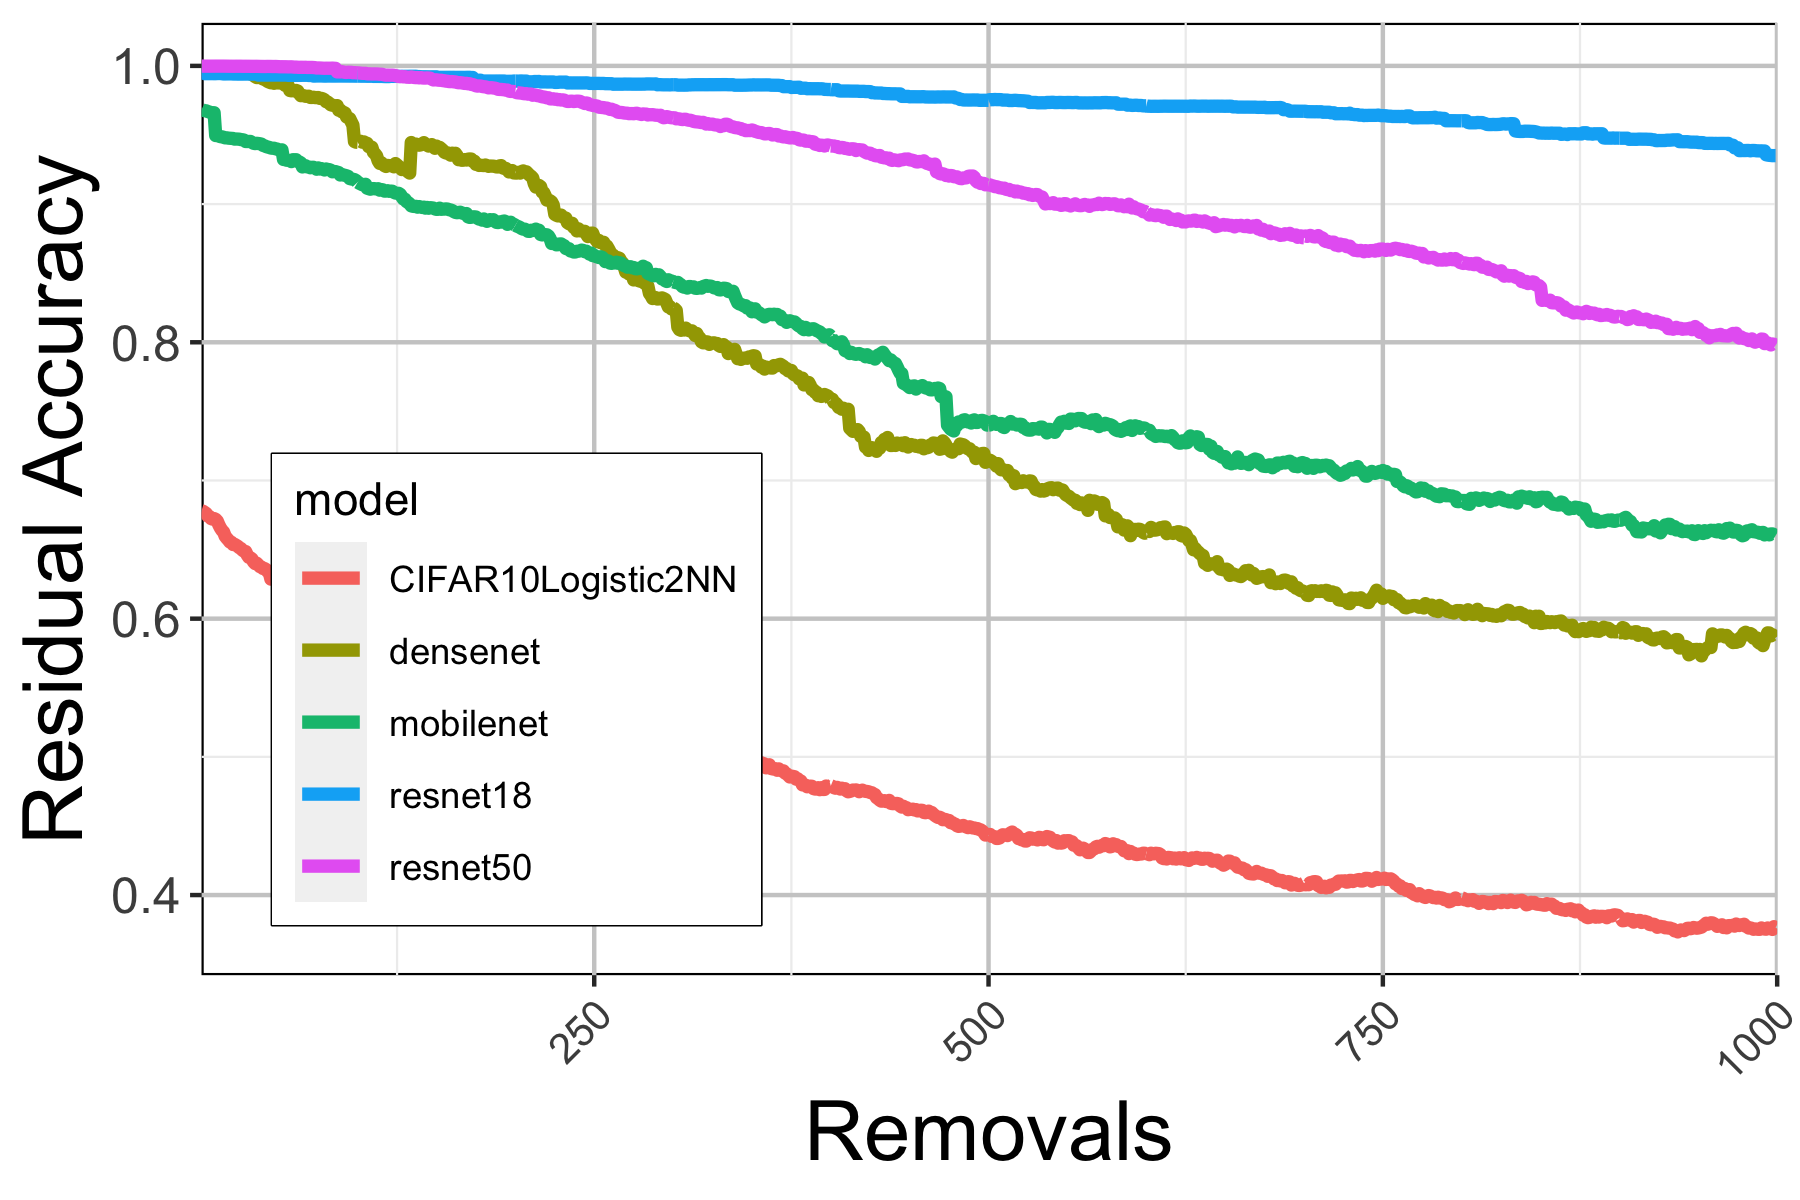
\includegraphics[width=0.24\textwidth]{5_unlearn/figs/scrub/cifar_resid.png}
    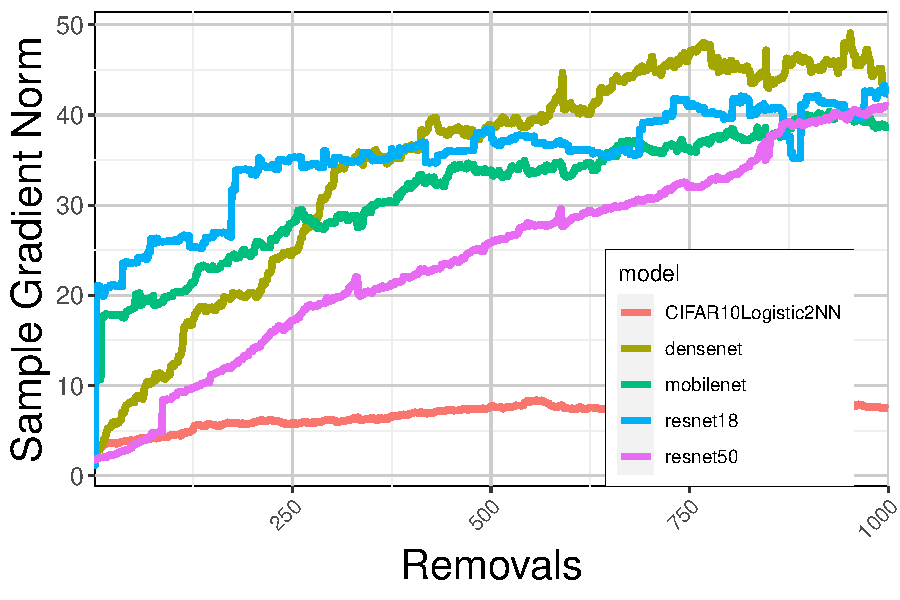
\includegraphics[width=0.24\textwidth]{5_unlearn/figs/scrub/CIFAR_gradnom.png}
    % \vspace{-8pt}
    \caption{(Left) Residual Accuracies \& Sample Gradient Norm of removal for an MNIST Logistic Regressor. Averaged over 10 runs. (Right) Residual accuracies and sample gradient norms for various CIFAR-10 models.}
    \label{fig:mnistcifar}
\end{figure*}


\paragraph{Are we selecting reasonable subsets?} A natural question is whether the subset selection via L-FOCI is any better than random, given that we are effectively taking a smaller global step. We answer this in the affirmative with a simple comparison with a random selection of size equal to the set selected by L-FOCI. Fig.~\ref{fig:mnistcifar} (left) shows that the sample gradient norm for selections made by L-FOCI are larger than those of a random selection: the subset of the model scrubbed of this specific sample has a larger impact on its final loss, and thus the gradient norm post-removal is large.


% \subsubsection{$\epsilon$-Certified Removal} 
% While we focus on the population minimizer setting from \cite{sekhari2021remember}, we also demonstrate the efficacy of LFOCI as a drop-in tool for another common unlearning setting described in \cite{guo2019certified}: hen a model is trained in a particular manner, a direct Newton ascent step is sufficent to guarantee $\epsilon$-removal. 

% Large drops in validation and residual accuracy indicate that a set of parameters integral to the model's predictions overall have been updated significantly. This suggests that the sample scrubbed may be a ``support vector" for the model. When these samples are considered for scrubbing, the model may have to be retrained. 

\paragraph{Does the formulation scale?} We scrub random samples from various CIFAR-10 models, and evaluate  performance for the same set of hyperparameters. When the models are larger than logistic regression, it is infeasible to estimate the full Hessians, so 
we {\em must} use our L-FOCI selection update. Fig.~\ref{fig:mnistcifar} (right) shows removal performance over many typical models with varying sizes. Models that have higher base accuracies tend to support more removals before performance drops. This matches results for differentially private models: models that generalize well may not have overfit and thus may already be private, allowing ``fast'' forgetting.

% \begin{figure}
%     \centering
%     % \includegraphics[width=0.33\textwidth]{5_unlearn/5_unlearn/figs/scrub/cifar_val.png}
%     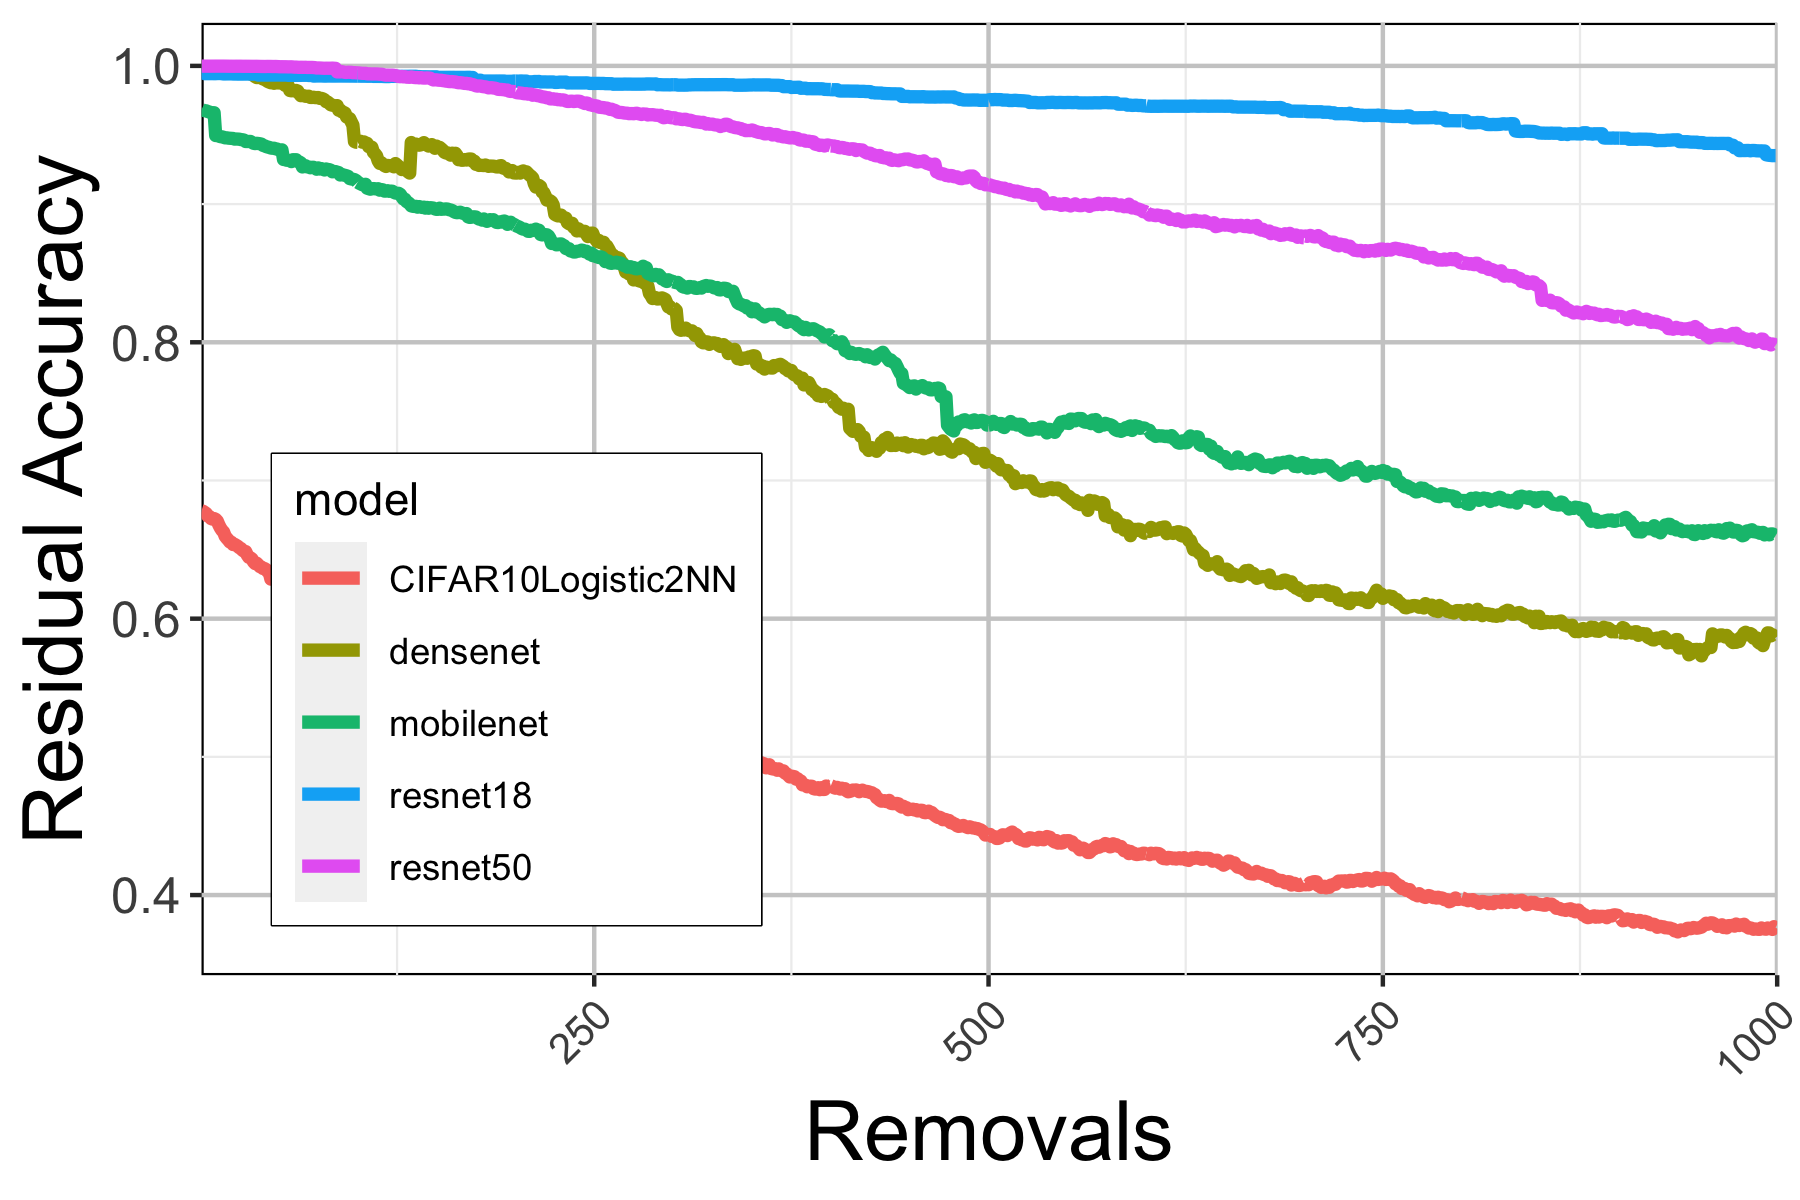
\includegraphics[width=0.49\columnwidth]{5_unlearn/figs/scrub/cifar_resid.pdf}
%     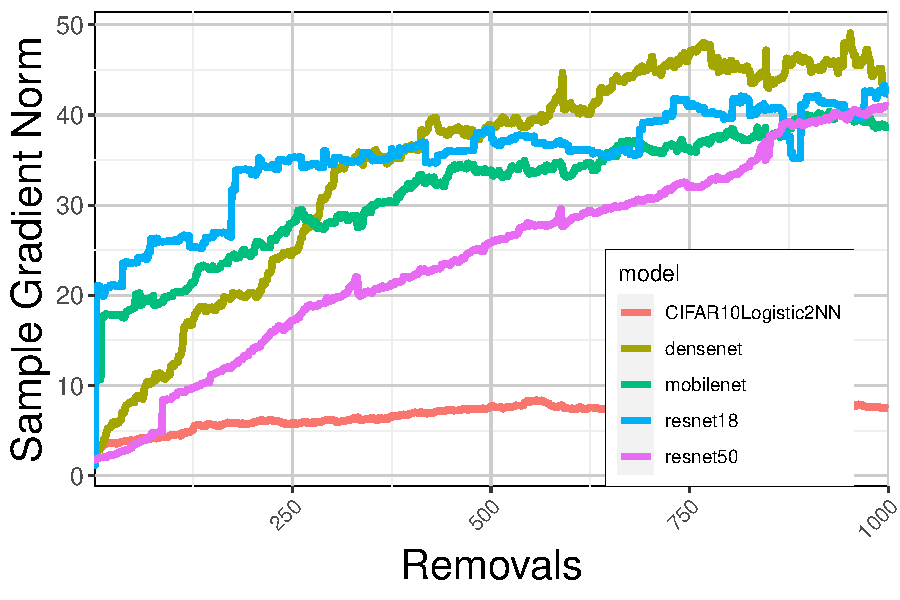
\includegraphics[width=0.49\columnwidth]{5_unlearn/figs/scrub/CIFAR_gradnom.pdf}
%     \vspace{-8pt}
%     \caption{Residual accuracies and sample gradient norms for various CIFAR-10 models.}
%     \label{fig:cifar}
% \end{figure}

\paragraph{Tradeoff vs Retraining.}
While our focus is the setting in which retraining is not feasible, where we can retrain we compare validation accuracies as a function of number of removals. Using a subset of MNIST, we train to convergence and iteratively remove samples using our construction, retraining fully at each step for comparison. With 1000 training samples from each class 
and reasonable settings of privacy parameters ($\epsilon=0.1,\delta=0.01$),
we support a large percentage of removals until validation accuracy drops more than a few percent, see Fig.~\ref{fig:retrain}.
\begin{figure}
    \centering
%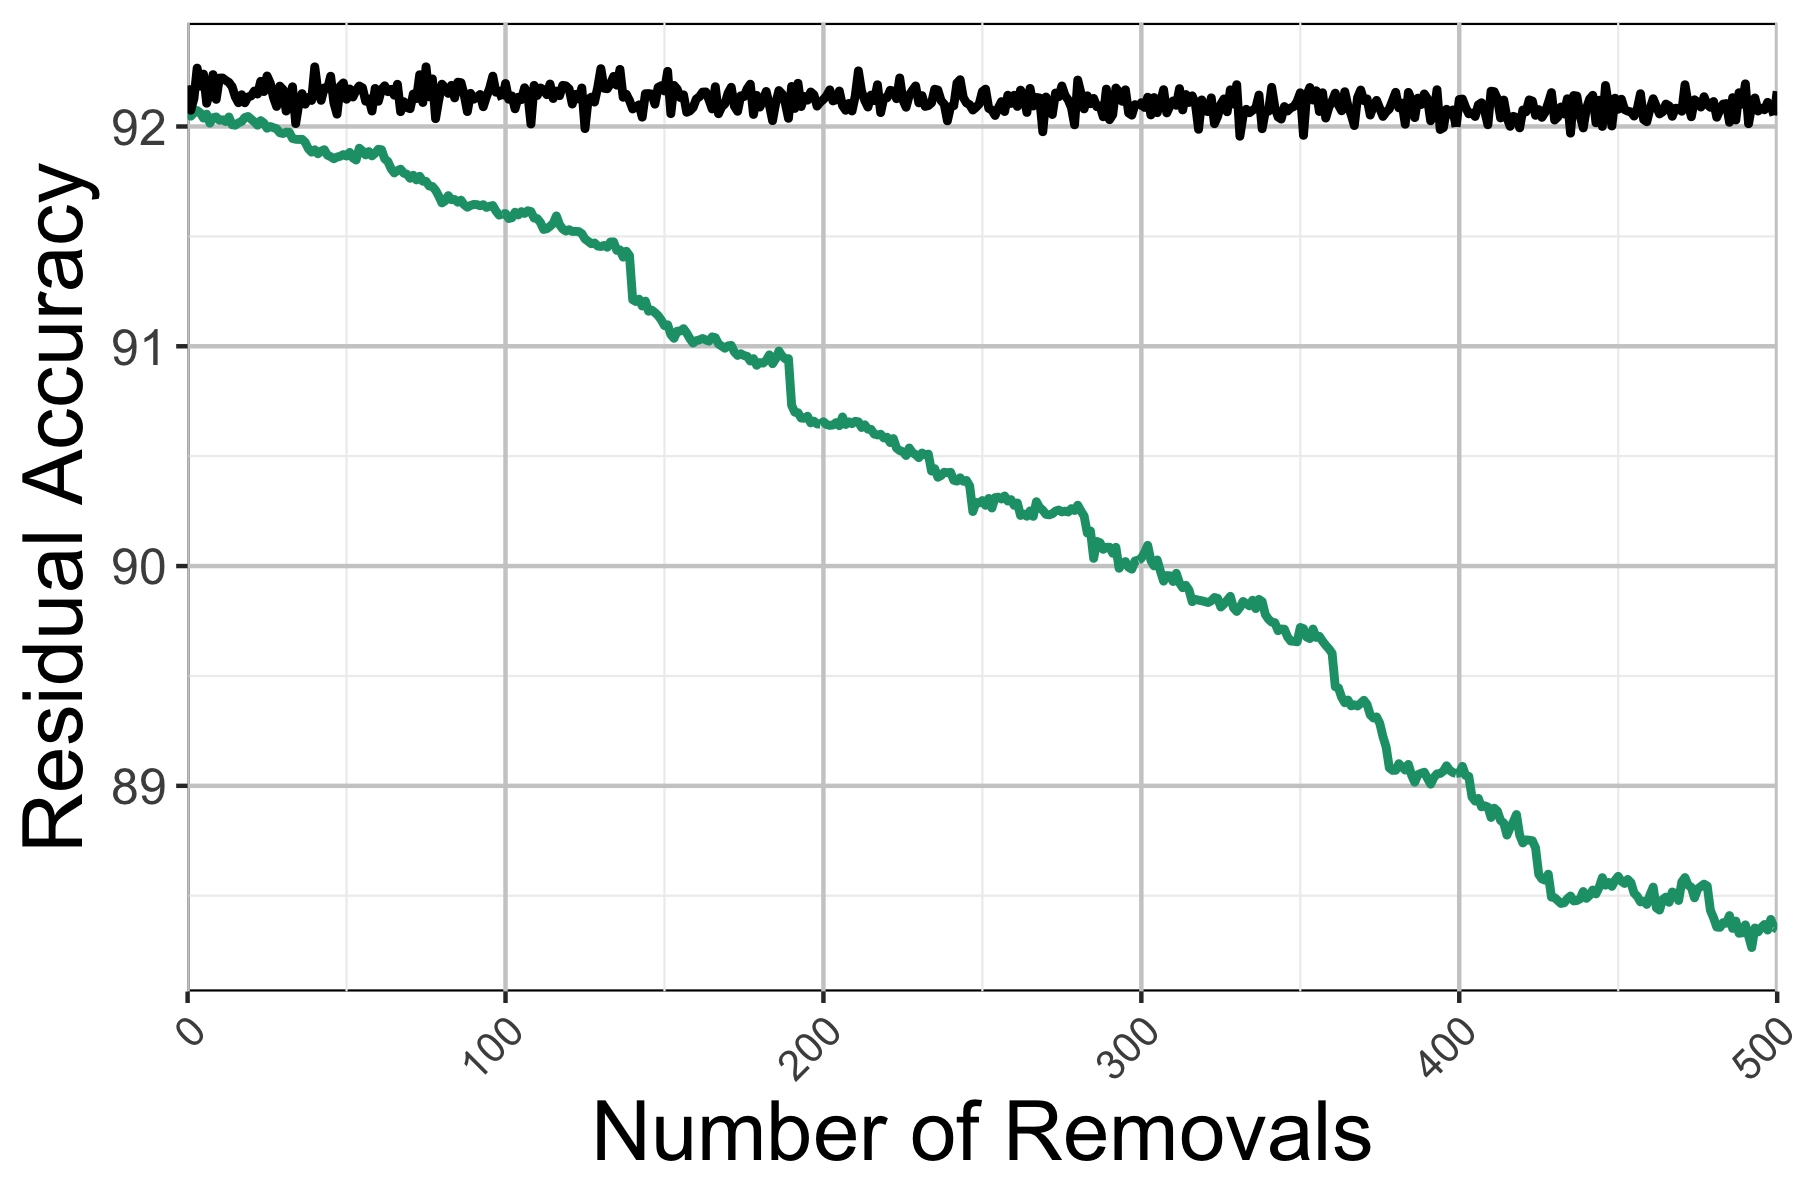
\includegraphics[width=0.31\columnwidth]{5_unlearn/figs/retrain/Retrain_Residual_Accs.png}
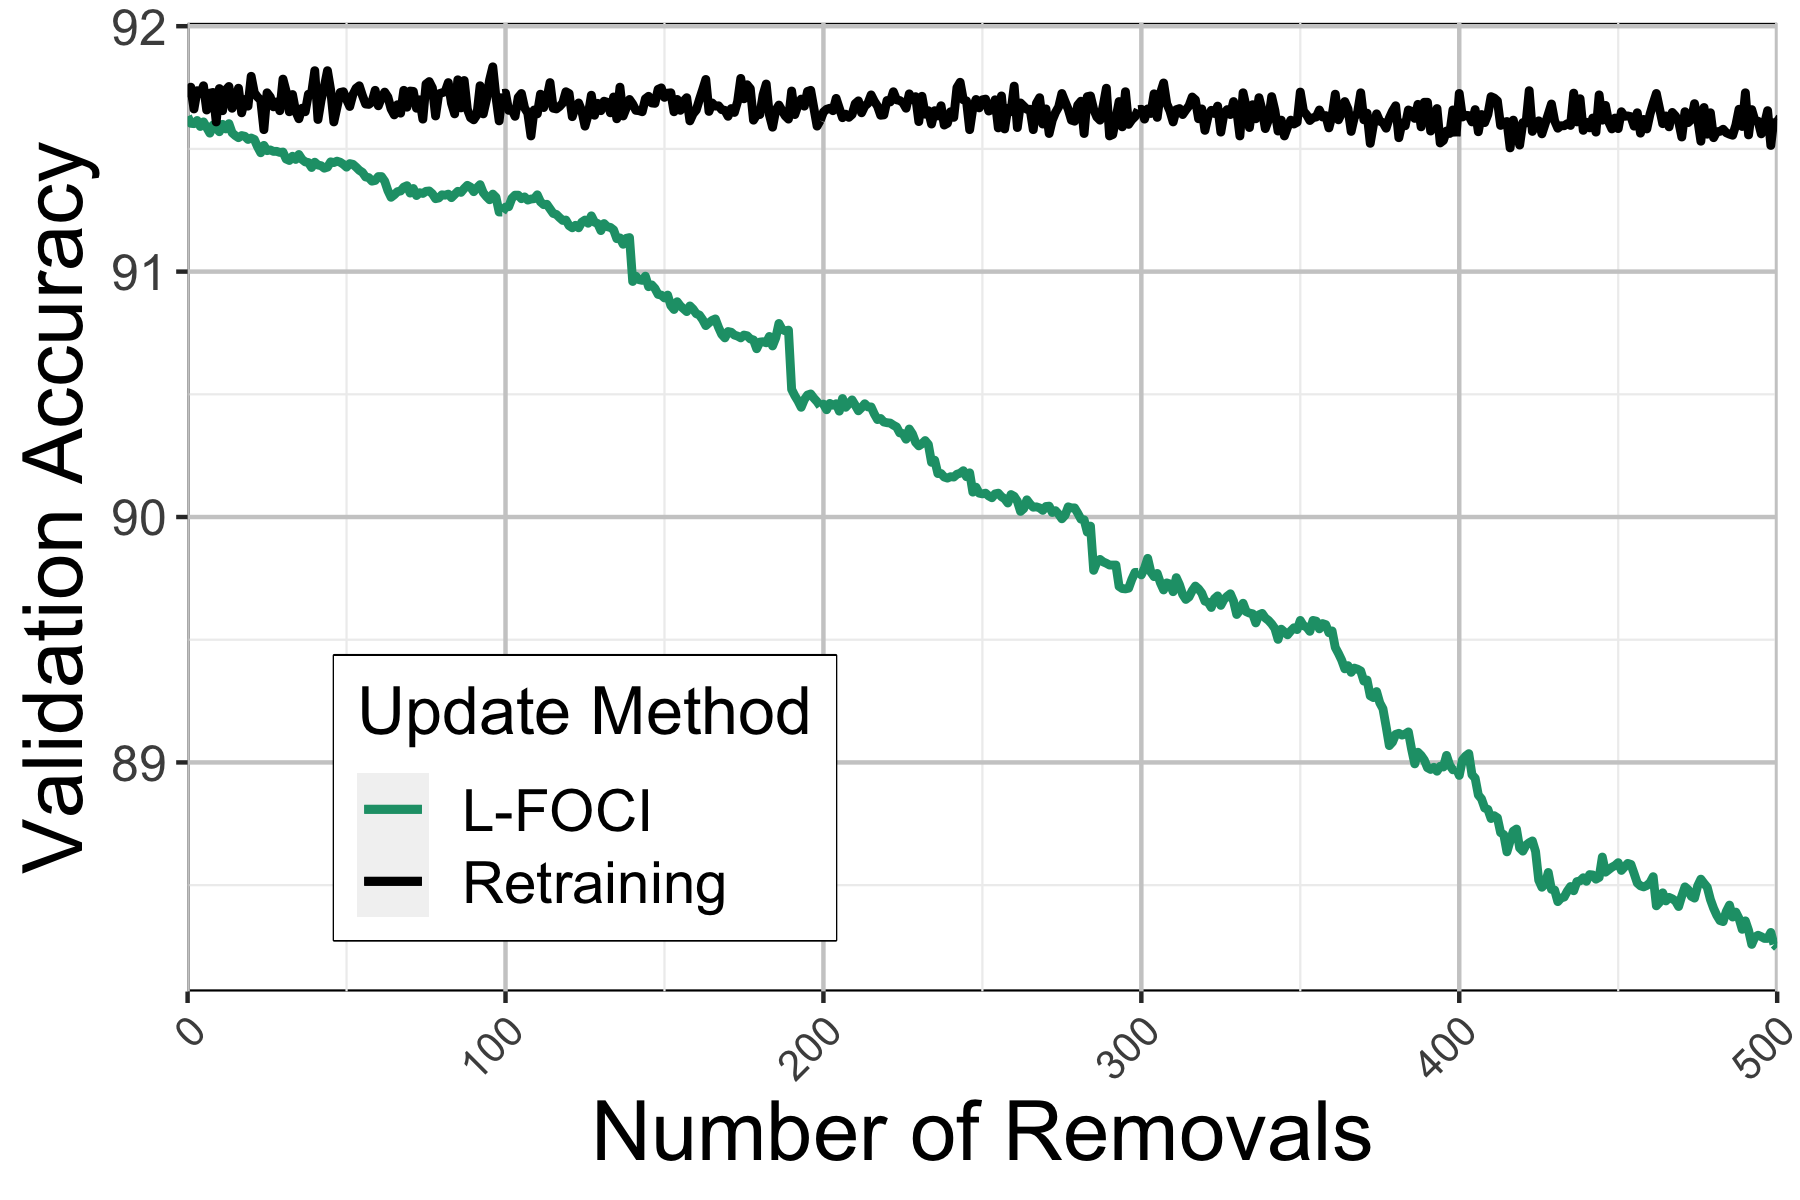
\includegraphics[width=0.49\columnwidth]{5_unlearn/figs/retrain/Retrain_Validation_Accs.png}
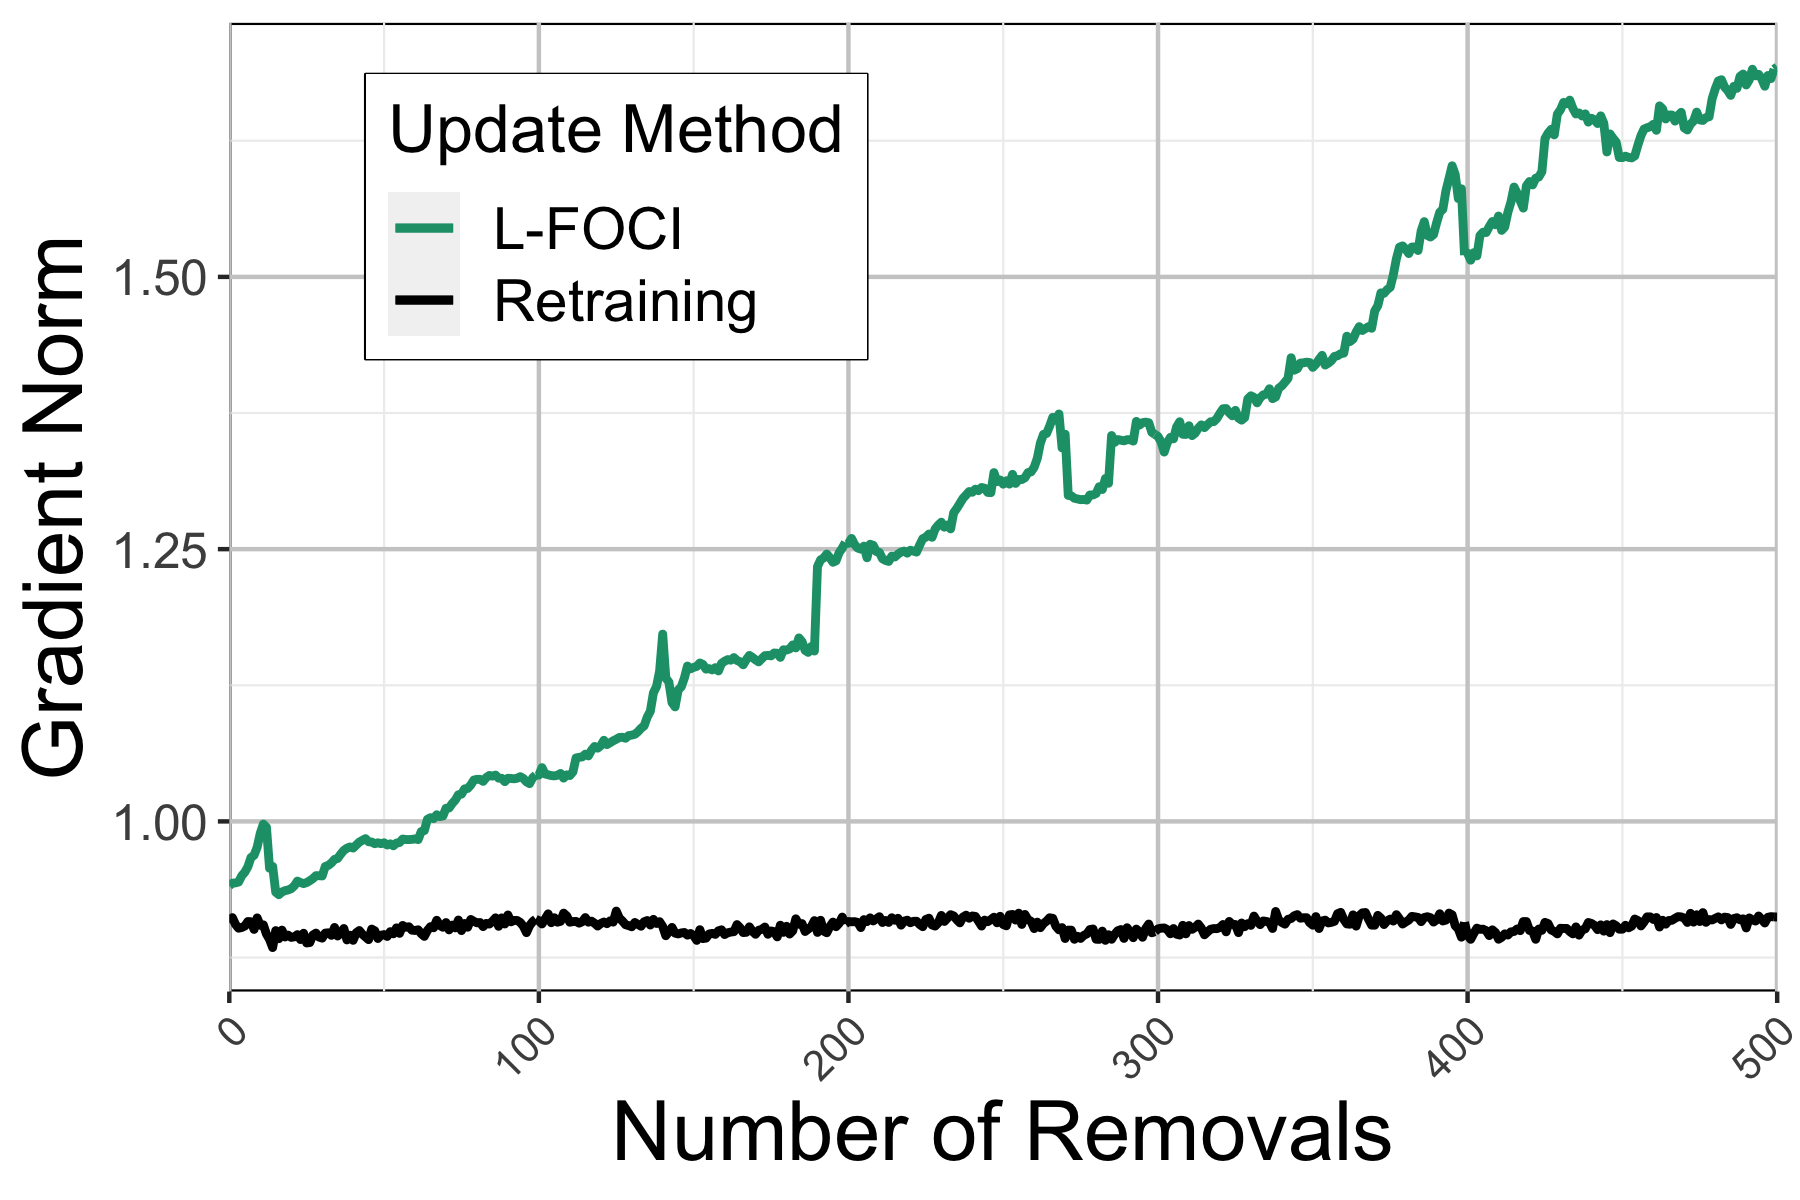
\includegraphics[width=0.49\columnwidth]{5_unlearn/figs/retrain/Retrain_Gradient_Norms.png}
    \caption{MNIST Retraining comparison averaged over 8 runs. Validation accuracies and residual gradient norms.}
    \label{fig:retrain}
\end{figure}

\subsection{Removal in NLP models}
We now scrub samples from transformer based models using  LEDGAR \cite{tuggener2020ledgar}, a multilabel corpus of legal provisions in contracts. We use the prototypical subset which contains $110156$ provisions pertaining to $13$ most commonly used labels based on frequency. Our model is a fine-tuned DistilBERT \cite{sanh2019distilbert} and uses the $[CLS]$ token as an input to the classification head. 
Table. \ref{tab:nlp} shows results of scrubbing the provisions from two different classes; \textit{Governing Laws} and \textit{Terminations} which have the highest/lowest support in the test set. As expected with increasing $\epsilon$, i.e., lower privacy guarantees, we can support more number of removals based on the Micro F1 score of the overall model. 
% {\color{red}The Micro F1 scores for the overall model, start to fall off after that of the class being removed and the change in overall scores is more gradual than that of the removal class. }
The Micro F1 scores, for the removed class fall off rapidly, while the change in overall scores is more gradual. 

% \begin{table}
%     \centering
%     \resizebox{!}{60pt}{%
%     \begin{tabular}[b]{l|ccc}
%         \hline\hline
%         & \multicolumn{2}{c}{\# Supported Removals}  \\
%         $\epsilon$ & Governing Laws & Terminations \\
%         \hline
%         0.1 & $>$ 100 & $>$ 100 \\
%         0.01 & $>$ 100 & $>$ 100 \\
%         0.001 & 18 & 21 \\
%         0.0005 & 6 & 7 \\
%         \hline\hline
%     \end{tabular}%
%     }
%     \vspace{-8pt}
%     \caption{\label{tab:nlp} Scrubbing transformer model for provision classification.}
% \end{table}

% \subsubsection{Appendix: Direct Application in existing CR Setting}
% using FOCI in a naive setting does not harm final result. (Equivalent to full when doing one vs. all, better than random).

\subsection{Removal from Pretrained Models}
The above settings show settings where a sample from one specific source may be removed. A more direct application of unlearning 
is completely removing samples from a specific class; a compelling use case is face recognition.

We utilize the VGGFace dataset and model, pretrained from the original work in \cite{huang2008labeled,Parkhi15}. The model uses a total of approximately 1 million images to predict the identity of 2622 celebrities in the dataset. Using a reconstructed subset of 100 images from each person, we first fine-tune the model on this subset for 5 epochs, and use the resultant models as estimates of the Hessian. 
In this setting, the VGGFace model is very large, including a linear layer of size $25088 \times 4096$. Selecting even a few slices from this layer results in a Hessian matrix unable to fit in typical memory. For this reason, we run a ``cheap" version of L-FOCI: we select only one slice that results in the largest conditional dependence on the output loss.
%
% \begin{figure}
%     \centering
%     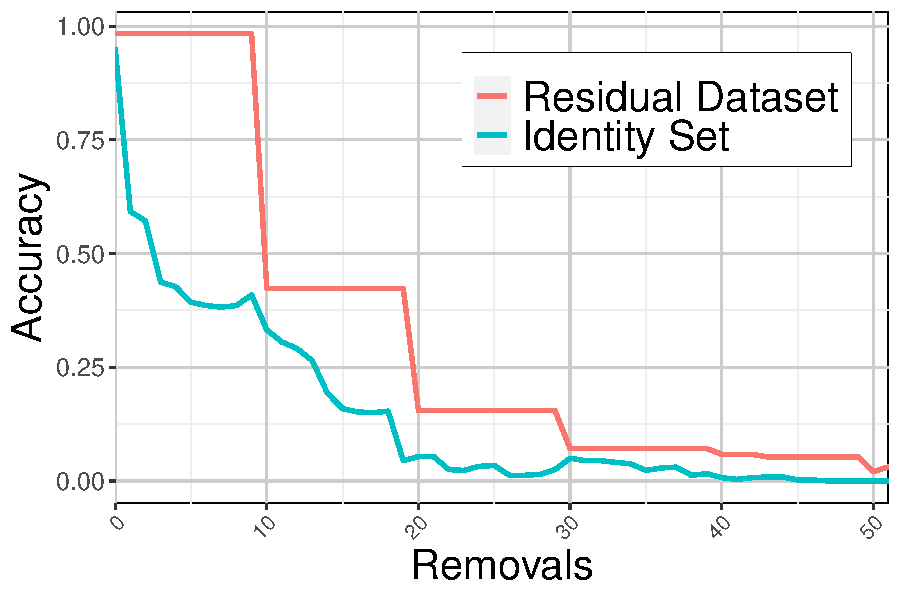
\includegraphics[width=0.5\columnwidth]{5_unlearn/figs/scrub/VGG_Scrub_1.pdf}
%     \vspace{-10pt}
%     \caption{Accuracies on scrubbed class and Residual Sample Sets (every 10 removals) for $\epsilon = 1e^{-5}$. The accuracy drop for the residual set is gradual up to a certain number of removals.}
%     \label{fig:vgg}
% \end{figure}


\stepcounter{table}
\begin{figure}
\begin{subfigure}{0.45\columnwidth}\centering
    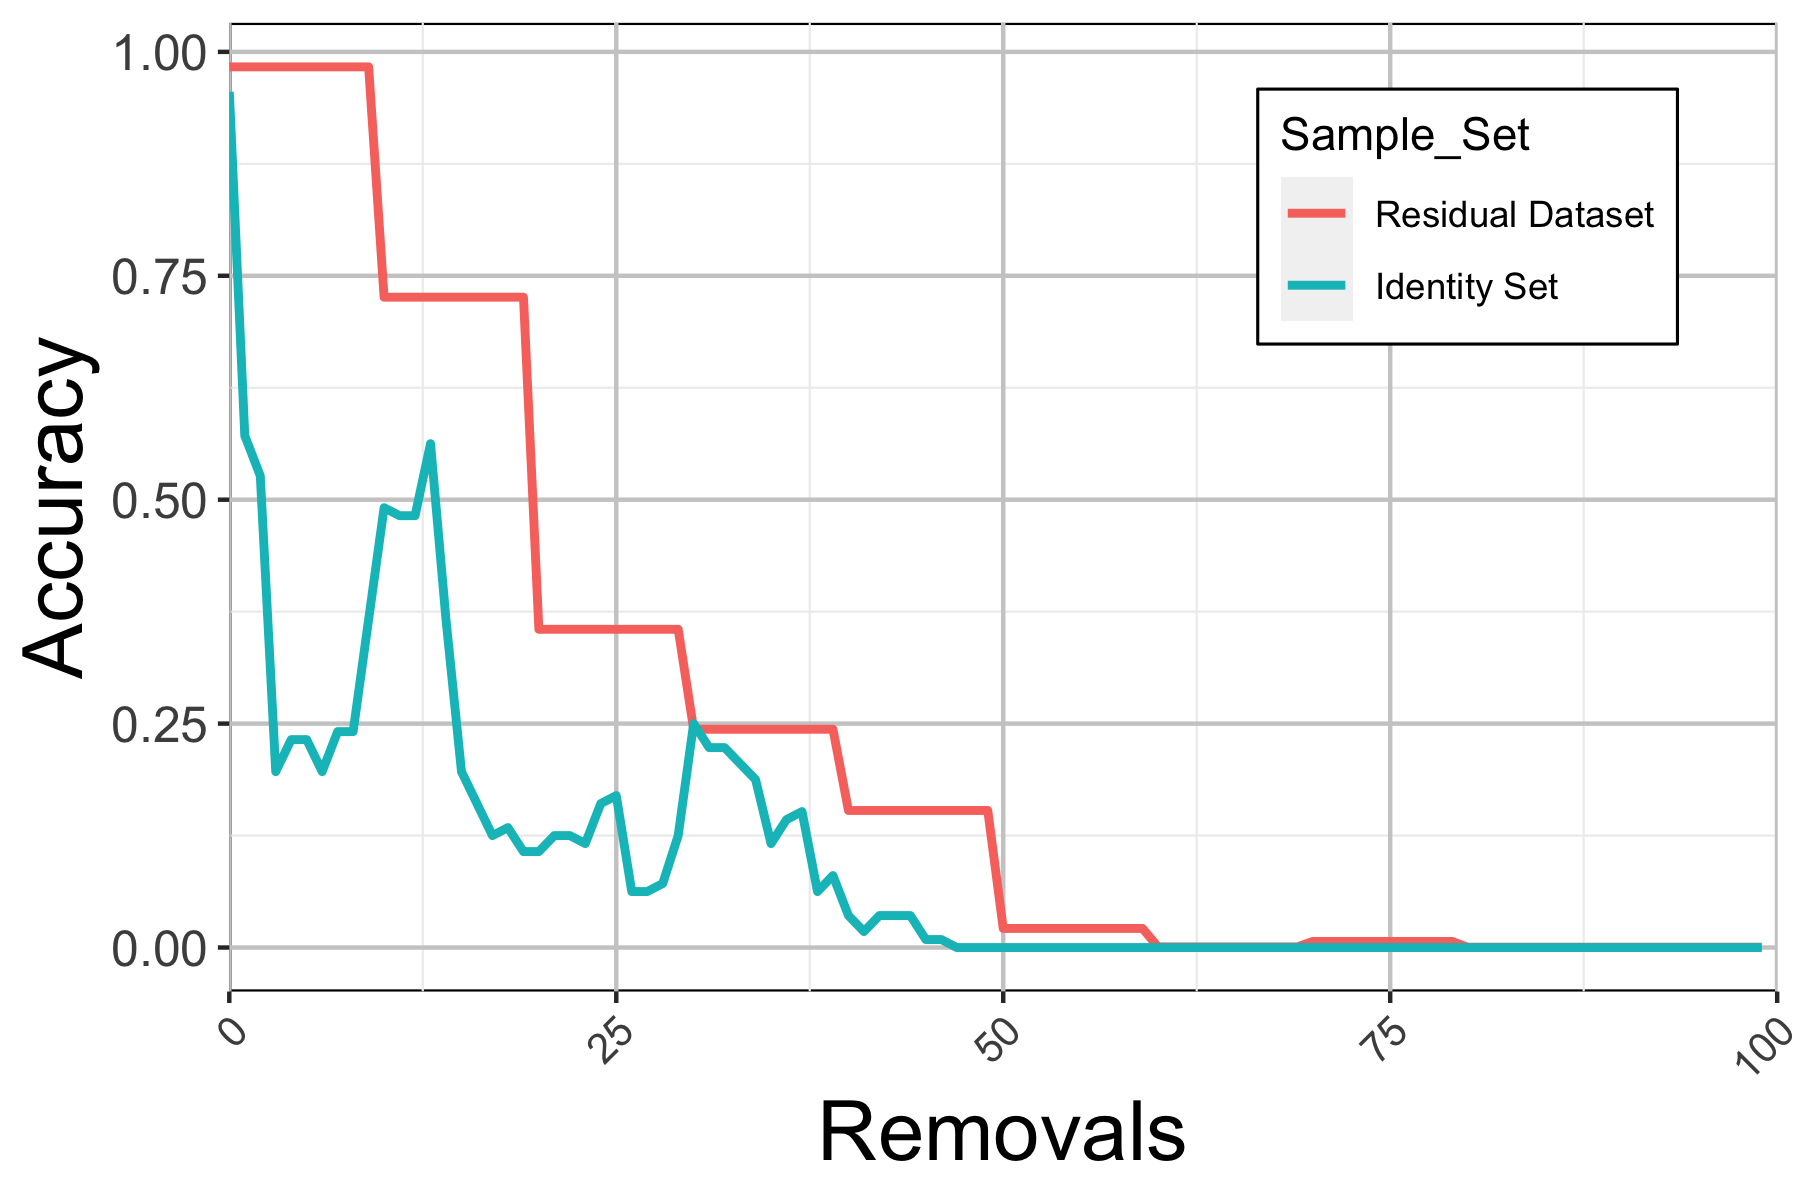
\includegraphics[width=0.98\columnwidth]{5_unlearn/figs/scrub/VGG_Scrub_1.png}%
    \phantomsubcaption
    \label{fig:vgg}
\end{subfigure}
\begin{subfigure}{0.495\columnwidth}
    \centering
    \resizebox{!}{85pt}{%
    \begin{tabular}[b]{l|ccc}
        \hline\hline
        %& \multicolumn{2}{c}{}  \\
        & \multicolumn{2}{c}{\# Supported Removals}  \\
        $\epsilon$ & Governing Laws & Terminations \\
        \hline
        0.1 & $>$ 100 & $>$ 100 \\
        0.01 & $>$ 100 & $>$ 100 \\
        0.001 & 18 & 21 \\
        0.0005 & 6 & 7 \\
        \hline\hline
    \end{tabular}%
    }
    \phantomsubcaption
    \label{tab:nlp}
\end{subfigure}
%\captionsetup{labelformat=andtable}

\caption[important image]{(Left) Scrubbed and Residual Accuracies (every 10 removals) for $\epsilon = 1e^{-5}$. The accuracy drop for the residual set is gradual up to a certain number of removals. (Right) Scrubbing transformer model for provision classification.}
\label{fig:combine}
\vspace{-5pt}
\end{figure}

Fig.~\ref{fig:vgg} show results for scrubbing consecutive images from one individual in the dataset for a strong privacy guarantee of $\epsilon=10^{-5}$. As the number of samples scrubbed increases, the performance on that class drops faster than on the residual set, exactly as desired.

\subsection{Removal from Person re-identification model}
As a natural extension to our experiments on face recognition, we evaluate unlearning of deep neural networks trained for person re-identification. Here, the task is to associate the images pertaining to a particular individual but collected in diverse camera settings, both belonging to the same camera or from multiple cameras. In our experiments, we use the Market-1501 dataset \cite{zheng2015scalable} and a Resnet50 architecture which was trained for the task. We unlearn samples belonging to a particular person, one at a time, and check the performance of the model. Experimental results are in agreement with results reported for the transformer model as well as the VGGFace model. With very small values of $\epsilon$ i.e. $0.0005$ the number of supported removals is limited to less than $10$ depending on the person id being removed. However, with a larger value of $\epsilon$, e.g., $0.1$, all potential samples can be removed without a noticeable degradation in model performance in terms of mAP scores. In Fig.~\ref{fig:reid}, we clearly see that after scrubbing a model for a particular person, its predictions for that particular individual become meaningless whereas the predictions on other classes are still possible with confidence, as desired. Additional experiments with different datasets, model architectures and other ablations for deep unlearning for person re-identification models are presented in the appendix.

\begin{figure}[!tb]
    \centering
    %\includegraphics[width=0.3\textwidth]{5_unlearn/figs/scrub/MNIST_Valid_Acc.png}
    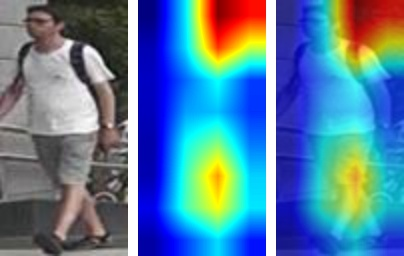
\includegraphics[width=0.49\columnwidth]{5_unlearn/figs/scrub/0006_c3s3_075694_00.jpg}
     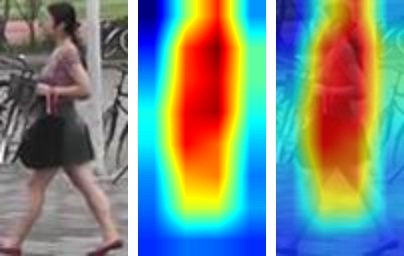
\includegraphics[width=0.49\columnwidth]{5_unlearn/figs/scrub/0101_c5s1_021926_00.jpg}
    \caption{\label{fig:reid}Activation maps from a model scrubbed for the person on the left (right set is not scrubbed). For each triplet, from (L to R) are the original image, the activation map and its image overlay. Note the effect of scrubbing: activations change significantly for the scrubbed sample (compare column 2 to 3) whereas remain stable for the non-scrubbed sample (compare column 5 to 6).}
\end{figure}

% \subsubsection{Scrubbing Reveals Sample Influence.}
% Observe in some of above results there are some significantly large changes in sample gradient norms, corresponding to large drops in residual and validation accuracy. These may indicate highly influential samples, in the sense that they may represent ``support vectors" for the model. For dataset X, we show a few of these identified in Figure~\ref{fig:samps}. Qualitatively these appear to be reasonably unique samples for their particular class. While this is observation appears reasonable, the direct connection to sample influence in the traditional sense remains open for future work.


% \begin{figure}
%     \centering
%     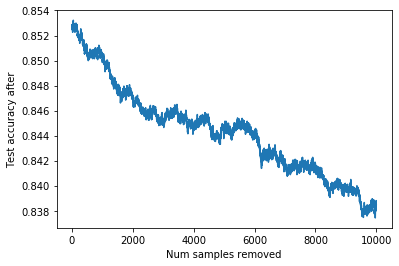
\includegraphics[width=0.22\textwidth]{5_unlearn/figs/scrub/custom_full_acc.png}
%     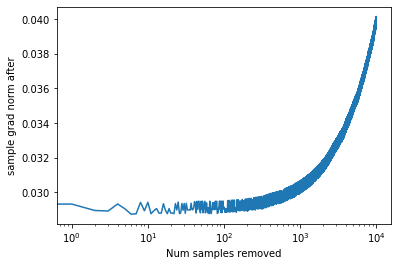
\includegraphics[width=0.22\textwidth]{5_unlearn/figs/scrub/custom_full_grad.png}
%     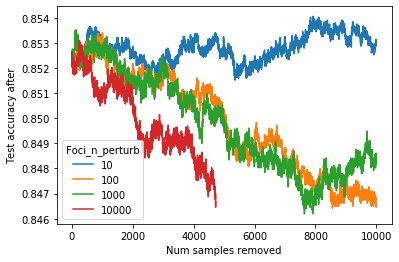
\includegraphics[width=0.22\textwidth]{5_unlearn/figs/scrub/custom_foci_acc.png}
%     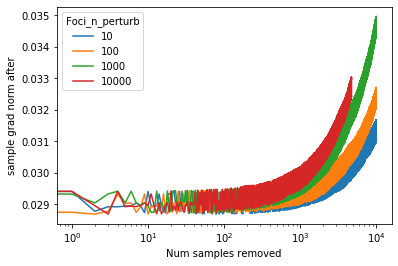
\includegraphics[width=0.22\textwidth]{5_unlearn/figs/scrub/custom_foci_grad.png}
%     \caption{scrubbing results, spectrum before and after.}
%     \label{fig:scrub_res}
%     \caption{\ronak{These plots will be replaced with results from "comparing with full Hesian".}}
% \end{figure}





%%% Older writing, to be moved/incorporated.
% \subsection{Older writing, to be moved/incorporated.}
% With the above proofs-of-concept in hand, we move to evaluating the full unlearning procedure on larger neural network models.


% We compare our L-FOCI unlearning procedure against a full Hessian step as in \cite{sekhari2021remember}, using a simple XXX model trained on CIFAR-10 such that the computation is feasible. 

% \paragraph{Implementation Details.} Our selection procedure is implemented in PyTorch, with a framework for mapping and vectorizing convolutional layers and filters selected by L-FOCI over hypercolumns. Hessians are approximated using finite-differencing, and computed using the gradient vectors at the last two epochs of training. Full experimental details along with code for our experiments can be found in the supplement.

% \begin{figure}
%     \centering
%     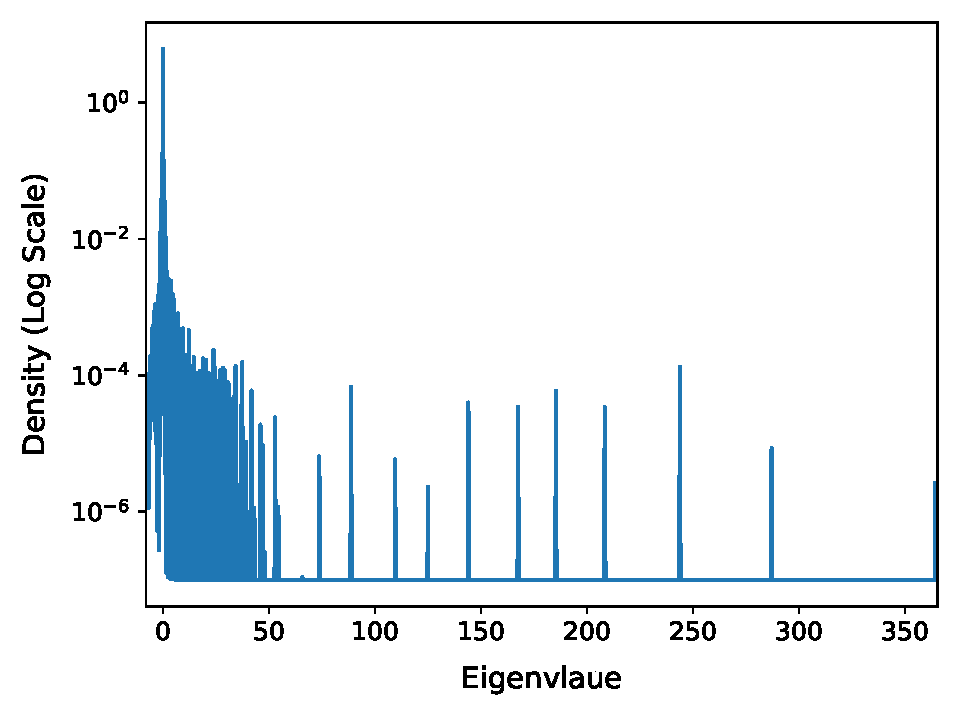
\includegraphics[width=0.22\textwidth]{5_unlearn/figs/spectra/cifar10_simple_before_train.pdf}
%     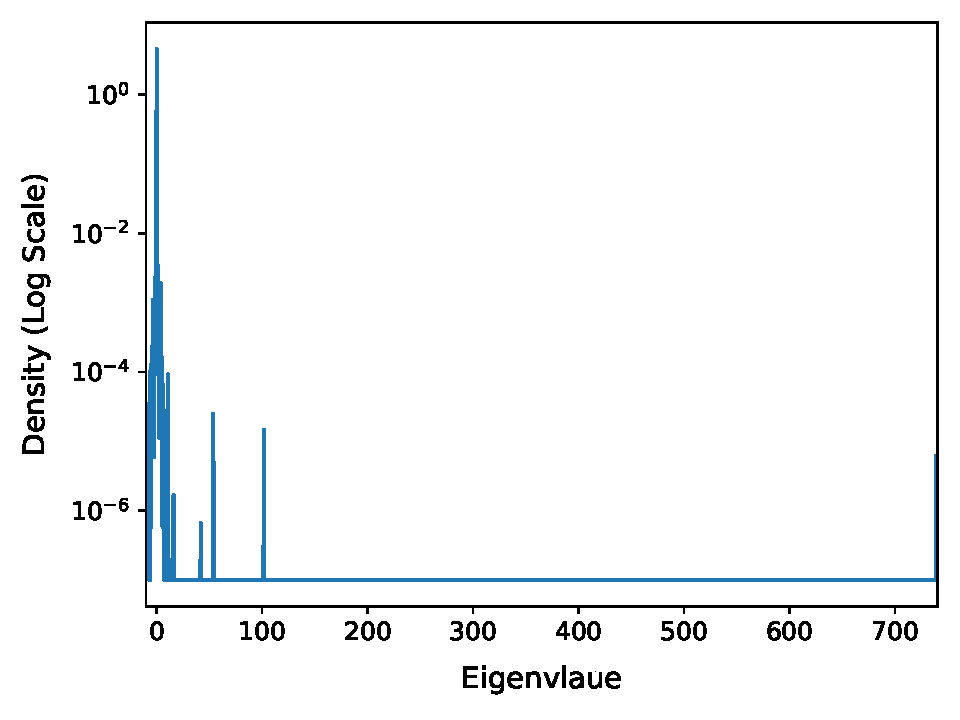
\includegraphics[width=0.22\textwidth]{5_unlearn/figs/spectra/cifar10_simple_after_14.pdf}
%     \caption{\ronak{TODO: update with newer version, fixed models.}}
%     \label{fig:my_label}
% \end{figure}

% \paragraph{Unlearning Setup.} Here, we compare our L-FOCI unlearning procedure against a full Hessian step. We train a ResNet-20 model on CIFAR-10. While the model is large, we are still able to compute the full Hessian update.
%  {\color{red} TODO: model, transforms, learning rate/epochs, etc. }

% \paragraph{Baseline ablations.} {\color{red} if smaller model for full Hessian approx, details here}. Using the model above, we evaluate and compare various unlearning procedures. Table~\ref{tab:scrub} shows gradient norms and validation accuracies before and after scrubbing using naive methods of simple backpropogation, full Hessian updates as in \cite{sekhari2021remember}, random selections of layers, and selections via L-FOCI.

% \paragraph{Spectral analysis.} Using \cite{yao2020pyhessian}, we can quickly approximate the second-order eigenspectrum of a model at specific points in the input space.
%In Figure~\ref{fig:eigen}, we show the spectra of the baseline model above before and after scrubbing 


% \paragraph{Convergence.} If we have time run multiple steps, show spectrum changing?



% \subsubsection{Unlearning Identities in CelebA}
% person identification, exposing AI, data use...

% exp setup: n classes, model for IDing, scrubbing a person means scrubbing all of their images, accuracy for classification on that person decreases.



% \subsubsection{Estimating Sample Influence}
% \begin{outline}[enumerate]
% \1 identifying important samples in traditional classification
%     \2 to use FSI, need to fall back to weight 2-norm
%     \2 MNIST
%     \2 Identifying OOD/Corrupted Samples
%         \3 plots of in/out distribution a la soatto
%     \2 minimal sets for accuracy
%         \3 redo soatto plot
% \end{outline}